\documentclass[11pt]{article}

% ---------------- packages ----------------
\usepackage[utf8]{inputenc}
\usepackage[T1]{fontenc}
\usepackage{lmodern}
\usepackage[a4paper,margin=1in]{geometry}
\usepackage{booktabs}
\usepackage{tabularx}
\usepackage{longtable}
\usepackage{multirow}
\usepackage{graphicx}
\usepackage{caption}
\usepackage{float}
\usepackage{authblk}
\usepackage{siunitx}
\usepackage{amsmath,amssymb}
\usepackage[hidelinks]{hyperref}
\usepackage{xcolor}
\usepackage[numbers,sort&compress]{natbib}
\setlength{\emergencystretch}{3em}

\captionsetup{labelfont=bf,font=small,skip=6pt}
\graphicspath{{figs/}}
\setlength{\parskip}{0.35em}
\renewcommand{\arraystretch}{1.15}

% ---------------- title ----------------
\title{\textbf{Can a zero-shot time-series foundation model rival
task-trained models for intraoperative hypotension prediction? A two-cohort
benchmark and the role of covariate-awareness}}

\author[1,2]{Max Haberbusch}
\affil[1]{Center for Medical Physics and Biomedical Engineering, Medical University of Vienna, Vienna, Austria}
\affil[2]{Ludwig Boltzmann Institute for Cardiovascular Research, Vienna, Austria}
\affil[ ]{\normalfont Correspondence: \texttt{max.haberbusch@meduniwien.ac.at}}
\date{}

\begin{document}
\maketitle

% ---------------- abstract ----------------
\begin{abstract}
\noindent
Intraoperative hypotension is common and linked to organ injury. Models that
forecast mean arterial pressure (MAP) are trained on large, site-specific
labelled cohorts, which limits portability. We asked whether general-purpose
time-series foundation models, applied zero-shot---no task-specific training,
no labels---can rival task-trained models. On 2{,}708 VitalDB cases we
benchmarked four zero-shot foundation models against task-trained Temporal
Fusion Transformer (TFT) and PatchTST baselines, predicting hypotension
(MAP\,$<$\,65~mmHg) over 1--15~min. TiRex-2 led all foundation models and
matched TFT at short-to-mid horizons (AUROC 0.929 vs 0.923 at 5~min) but
trailed the stronger PatchTST at longer horizons. Its lead held even without
the drug-infusion covariate, indicating base forecast quality. On an external
cohort (MOVER; 2--3$\times$ higher prevalence) the identical model held
AUROC\,$\geq$\,0.85 and matched MOVER-trained models. Zero-shot foundation
models are thus a portable alternative for intraoperative hypotension
prediction---matching TFT, though not the strongest supervised baseline.
\end{abstract}

\section{Introduction}

General anaesthesia perturbs cardiovascular physiology: hypnotics and
opioids reduce cardiac inotropy and systemic vascular resistance, and
intraoperative hypotension---commonly defined as a mean arterial pressure
(MAP) below 65~mmHg---is a frequent consequence \citep{Kapral2024,Zhu2026}.
Even brief exposure is associated with postoperative myocardial injury,
acute kidney injury and mortality
\citep{Walsh2013,Salmasi2017,Sun2015,Mascha2015,SesslerKhanna2018}, and
cumulative hypotension burden shows a dose-dependent association with organ
injury \citep{Zhu2026}. Because clinicians largely respond to hypotension
reactively, anticipating it minutes in advance could shift management from
reactive rescue to prevention \citep{Sessler2019,Wijnberge2020}.

Two lines of predictive work dominate. The first is the commercial
Hypotension Prediction Index (HPI), a machine-learning model built on
high-fidelity arterial-waveform features that flags impending hypotension
\citep{Hatib2018,Davies2020}. A randomised trial found HPI-guided care
reduced hypotension duration \citep{Wijnberge2020}, but the index requires
an invasive arterial waveform, and its reported performance has been
criticised for selection bias, with the suggestion that it may not surpass a
simple MAP alarm threshold of 70--75~mmHg
\citep{Enevoldsen2022,Vistisen2024}. The second line trains bespoke
deep-learning models on large, site-specific labelled cohorts. Two recent,
closely related models define the current state of the art and the principal comparators for
the present work. Kapral et al.\ trained a Temporal Fusion Transformer (TFT)
on 73{,}009 patients to forecast the continuous MAP trajectory 7~min ahead
and derive binary hypotension predictions, using low-resolution vital signs
together with intraoperative medication as an observed, past input; they
report an external mean absolute error (MAE) of 7~mmHg on VitalDB
\citep{Kapral2024}. Zhu et al.\ trained a Transformer on 319{,}699 cases to
classify impending hypotension at 5--15~min from vital signs alone,
deliberately excluding medication on the assumption that vital-sign dynamics
implicitly encode drug effects, and report internal area under the receiver
operating characteristic curve (AUROC) values of 0.904/\allowbreak0.892/\allowbreak0.882 at
5/10/15~min, attenuating to 0.897/\allowbreak0.862/\allowbreak0.822 on external VitalDB validation
\citep{Zhu2026}.

Both models share three properties that bound their portability and scope.
They require \emph{task-specific training on large labelled cohorts}---the
very site-specific labelled training set that limits transfer to new
institutions. They condition on the drug covariate as \emph{observed history
only, or not at all}: Kapral's model explicitly cannot use a drug given
after the prediction origin---as their own Fig.~1 caption states, ``as the
administration of phenylephrine occurs after the prediction start, it cannot
be taken into account for forecasting MAP''---and they attribute external
overestimation of hypotension to the model ``not anticipating future medical
interventions'' \citep{Kapral2024}. Zhu's model omits medication entirely
and asserts, but never tests, that vital signs implicitly capture it
\citep{Zhu2026}. And each is a \emph{single site-specific model}, not an
evaluation of a general modelling paradigm.

Meanwhile, time-series foundation models---large models pretrained on broad
corpora that forecast new series zero-shot, with no task-specific
training---have advanced rapidly (Chronos, TimesFM, Moirai, TiRex)
\citep{Ansari2024,Das2024,Woo2024,Auer2025}, paralleling the
generalist-model shift in medical AI \citep{Moor2023}. Their appeal for
clinical deployment is portability: one pretrained model, no site-specific
labels. Yet perioperative hemodynamic evaluation of these models is
essentially absent from the literature, and most of them are
univariate---they cannot ingest an exogenous covariate such as a
drug-infusion plan. Conditioning on \emph{known-future} inputs is standard
inside trained architectures such as the TFT \citep{Lim2021}, but its use in
a zero-shot foundation model on a clinical intervention has not been
reported.

In this study we ask whether the zero-shot foundation-model paradigm can
meet this clinical need. We evaluate foundation models as a class, rather
than proposing a single new architecture, because their promise for
perioperative deployment lies precisely in generality: one pretrained model,
applied across institutions without task-specific labels or retraining. We
pursue three objectives. First, we test whether zero-shot foundation models
can rival task-trained state of the art for intraoperative MAP forecasting
and impending-hypotension prediction. Second, we ask what distinguishes the
strongest exemplar, focusing on the ability to condition on the anaesthetic
infusion the clinician plans to deliver---a known-future signal that
existing models cannot use. Third, we ask whether these findings hold on an
independent cohort with a different sampling cadence, covariate set and
hypotension prevalence.

To do so, we benchmark four zero-shot foundation models on two intraoperative
cohorts. TiRex-2 serves as the covariate-aware exemplar---the only model in
our panel that conditions on both past and known-future covariates---and is
compared against three univariate zero-shot models and two task-trained
baselines (TFT, PatchTST). We find that the zero-shot paradigm is competitive
with supervised state of the art at the short, clinically urgent horizons;
that conditioning on the known future drug-infusion plan is what separates the
leading exemplar from the rest of the field; and that both results replicate
externally on a cohort with markedly higher hypotension prevalence. The
advance is the pairing of zero-shot operation with known-future
conditioning applied to a clinical intervention; that past drug data
improves a supervised MAP forecast has already been established
\citep{Kapral2024}, and is not our claim.

\section{Results}

\subsection{Study design and cohorts}

We forecast MAP from a 30-min context and predict impending hypotension
(MAP\,$<$\,65~mmHg) over horizons of 1, 3, 5, 7, 10 and 15~min, with a
rolling origin and case-clustered inference throughout
(Fig.~\ref{fig:design}a). The development cohort comprised 2{,}708 VitalDB
cases contributing 47{,}642 forecast windows (median age 61~y, 57\% male,
83\% American Society of Anesthesiologists (ASA) physical status I--II; Table~\ref{tab:cohort}). Hypotension prevalence within the
forecast window rose with horizon, from 5.4\% at 1~min to 18.4\% at 15~min.
The independent external cohort, MOVER \citep{Samad2023}, comprised 1{,}827
cases with an invasive arterial MAP source at 60~s cadence and 2--3$\times$ higher
hypotension prevalence (16.7\% at 1~min to 41.4\% at 15~min). The two
cohorts differ in sampling cadence, available covariates, population and
prevalence, and are reported stratified---never pooled
(Fig.~\ref{fig:design}b). Representative forecasts for steady, transition
and hypotensive-onset windows are shown in Fig.~\ref{fig:design}c.

\begin{figure}[t]
\centering
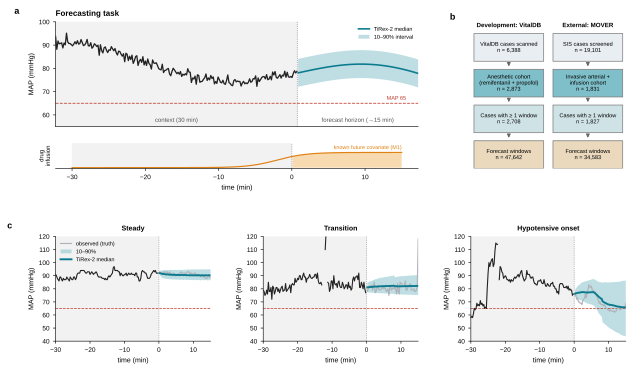
\includegraphics[width=\textwidth]{Fig1_design_cohort.png}
\caption{\textbf{Study design and two-cohort curation.}
(a)~Rolling-origin forecasting task: a 30-min context predicts MAP and
impending hypotension (MAP\,$<$\,65~mmHg) over 1--15~min.
(b)~Cohort curation funnel for the VitalDB development cohort and the
independent MOVER external cohort, which differ in cadence,
covariates and hypotension prevalence and are analysed stratified.
(c)~Representative forecasts for steady, transition and hypotensive-onset
windows.}
\label{fig:design}
\end{figure}

% ---------- Table 1 : Cohort characteristics ----------
\begin{table}[ht]
\centering\footnotesize
\caption{\textbf{Characteristics of the two cohorts} (cases contributing $\geq$1 forecast window). Hypotension prevalence is computed within the forecast window at each horizon. Both cohorts use an invasive arterial MAP source; they differ in sampling cadence (15 vs 60~s), available covariates and population. ASA physical status and surgical department are not recorded in the MOVER source tables.}
\label{tab:cohort}
\begin{tabularx}{\textwidth}{@{}l >{\raggedright\arraybackslash}X >{\raggedright\arraybackslash}X@{}}
\toprule
Characteristic & VitalDB (development) & MOVER (external) \\
\midrule
Cases, $n$ & 2{,}708 & 1{,}827 \\
Subjects, $n$ & 2{,}665 & 1{,}827 \\
Age, y --- median (IQR) & 61 (51--69) & 57 (45--68) \\
Male sex, $n$ (\%) & 1{,}555 (57\%) & 996 (55\%) \\
BMI, kg\,m$^{-2}$ --- median (IQR) & 23.0 (20.9--25.2) & 26.6 (23.1--31.2) \\
Anaesthesia duration, min --- median (IQR) & 235 (174--318) & 307 (212--418) \\
ASA I--II, $n$ (\%) & 2{,}254 (83\%) & --- \\
Top departments & General surgery 1629; Thoracic 912; Gynaecology 91 & --- \\
Sampling cadence & 15 s & 60 s \\
Forecast windows, $n$ & 47{,}642 & 34{,}583 \\
Hypotension prevalence @\,1 min, \% & 5.4 & 16.7 \\
Hypotension prevalence @\,5 min, \% & 10.6 & 28.1 \\
Hypotension prevalence @\,10 min, \% & 15.0 & 36.1 \\
Hypotension prevalence @\,15 min, \% & 18.4 & 41.4 \\
\bottomrule
\end{tabularx}
\end{table}

Zero-shot foundation models require no training and are inherently held out.
The task-trained baselines (TFT \citep{Lim2021}, PatchTST \citep{Nie2023})
were evaluated on all cases by
subject-level 5-fold out-of-fold cross-validation---each case predicted only
by the fold in which it was held out---and all models were scored on
identical windows with the same metric code. Per-fold learning curves
confirm convergence without overfitting on both cohorts
(Supplementary Fig.~\ref{fig:training_curves}).

\subsection{TiRex-2 leads every other zero-shot foundation model}
\label{sec:zeroshot}

We first benchmarked the four foundation models against one another, applied
zero-shot on identical held-out subjects, to identify the strongest exemplar
to carry forward. TiRex-2 had the highest hypotension AUROC at every horizon
(Table~\ref{tab:zeroshot}; Fig.~\ref{fig:zeroshot}). From 3~min onward the
lead over Chronos-Bolt, TimesFM-2.5 and Moirai-1.1-R was small but consistent
and statistically significant on case-clustered bootstrap paired tests: at
5~min, $+0.007$ vs Chronos-Bolt, $+0.008$ vs TimesFM-2.5 and $+0.007$ vs
Moirai-1.1-R (all $p<0.001$; Supplementary Table~\ref{tab:fm_pairwise}), and
the lead persisted through 10 and 15~min (e.g.\ $+0.012$ vs Moirai-1.1-R at
15~min). At the 1-min horizon the models were effectively tied---TiRex-2 was
indistinguishable from TimesFM-2.5 ($-0.0004$, $p=0.64$) and only marginally
ahead of Chronos-Bolt ($+0.001$, $p=0.009$)---so the separation among
foundation models emerges as the horizon lengthens rather than at the
shortest, most autocorrelated horizon. TiRex-2 also led on the continuous
ranked probability score (CRPS), on calibration at 10~min, and on the area
under the precision--recall curve (AUPRC) across horizons
(Fig.~\ref{fig:zeroshot}a--d).

This lead is not an artefact of TiRex-2's covariate access: even in its
covariate-free configuration, TiRex-2 matched or exceeded the univariate
models (5-min AUROC 0.925 vs 0.921 Chronos-Bolt, 0.920 TimesFM-2.5, 0.922
Moirai-1.1-R). TiRex-2 is therefore the strongest zero-shot forecaster in the
panel on its own merits, and it is additionally the only model able to ingest
the known-future drug-infusion covariate---the three univariate comparators
forecast covariate-blind by construction. We carry TiRex-2 forward as the
exemplar for the comparison against task-trained models and for the covariate
analysis.

\begin{figure}[t]
\centering
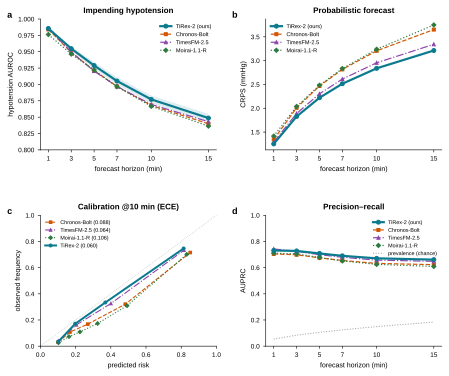
\includegraphics[width=\textwidth]{Fig3_zeroshot_tsfm.png}
\caption{\textbf{Zero-shot foundation-model benchmark on VitalDB.} TiRex-2
versus Chronos-Bolt, TimesFM-2.5 and Moirai-1.1-R on (a)~hypotension AUROC,
(b)~CRPS, (c)~calibration and (d)~AUPRC across horizons. Only TiRex-2
conditions on the known-future drug covariate.}
\label{fig:zeroshot}
\end{figure}

% ---------- Table 6 : Zero-shot foundation-model AUROC (VitalDB) ----------
\begin{table}[ht]
\centering\footnotesize
\caption{\textbf{Matched hypotension AUROC among zero-shot time-series foundation models on VitalDB} ($n=2{,}665$ subjects). All evaluated zero-shot; only TiRex-2 ingests the known-future drug-infusion covariate. Cells give AUROC with case-clustered bootstrap 95\% CI in brackets; bold marks the best model at each horizon.}
\label{tab:zeroshot}
\begin{tabular}{lcccc}
\toprule
Horizon (min) & TiRex-2 & Chronos-Bolt & TimesFM-2.5 & Moirai-1.1-R \\
\midrule
1  & \textbf{0.986} [0.984, 0.987] & 0.984 [0.982, 0.986] & \textbf{0.986} [0.984, 0.987] & 0.976 [0.973, 0.979] \\
3  & \textbf{0.955} [0.951, 0.958] & 0.949 [0.945, 0.953] & 0.950 [0.946, 0.954] & 0.946 [0.942, 0.951] \\
5  & \textbf{0.929} [0.924, 0.934] & 0.921 [0.916, 0.927] & 0.920 [0.915, 0.926] & 0.922 [0.917, 0.927] \\
7  & \textbf{0.905} [0.900, 0.911] & 0.897 [0.891, 0.903] & 0.897 [0.891, 0.903] & 0.897 [0.891, 0.903] \\
10 & \textbf{0.877} [0.871, 0.883] & 0.868 [0.861, 0.874] & 0.869 [0.863, 0.876] & 0.867 [0.860, 0.873] \\
15 & \textbf{0.849} [0.842, 0.855] & 0.840 [0.833, 0.846] & 0.843 [0.837, 0.850] & 0.836 [0.830, 0.843] \\
\bottomrule
\end{tabular}
\end{table}

\subsection{Zero-shot TiRex-2 matches TFT at short-to-mid horizons}

On VitalDB, zero-shot TiRex-2 matched the task-trained TFT baseline for
impending-hypotension discrimination at the short-to-mid horizons and was
competitive with, though below, the stronger PatchTST
(Table~\ref{tab:matched}; Fig.~\ref{fig:sota}). At 1~min TiRex-2
reached AUROC 0.986 (95\% CI 0.984--0.987), exceeding TFT (0.982) and
PatchTST (0.983); at 5~min it reached 0.929 (0.924--0.934), slightly but
significantly exceeding TFT (0.923; paired difference $+0.006$, $p=0.002$) while
trailing the stronger PatchTST (0.937; $-0.008$, $p<0.001$). At 7~min TiRex-2
(0.905) was statistically indistinguishable from TFT (0.903; $+0.002$,
$p=0.337$)---the point at which the two are a genuine match---while remaining
below PatchTST (0.918). Relative to TFT the task-trained model
pulled ahead only at the longest horizons (TiRex-2 below TFT by 0.011 at
15~min, $p<0.001$); relative to PatchTST, TiRex-2 trailed from 5~min onward
($-0.026$ at 15~min, $p<0.001$; Table~\ref{tab:stats}). The ``match'' is thus
specifically against TFT across 1--7~min, not against the best supervised
model across the full range.
For probabilistic forecasting accuracy (Supplementary Table~\ref{tab:forecast}), TiRex-2
had the lowest CRPS at 1~min (1.251 vs 1.311 TFT, 1.281 PatchTST) and
competitive MAE (3.03~mmHg at 1~min); the trained models achieved lower
error at longer horizons (e.g.\ 15-min MAE 7.95 vs 6.68~mmHg for PatchTST).
The pattern is consistent: a model that never saw a training label from this
task matches models trained on it precisely in the window where an
intraoperative warning is most actionable, and concedes ground only as the
horizon lengthens.

To calibrate these numbers against the autocorrelation of MAP, we added a
naive persistence baseline that ranks impending hypotension by the last
observed MAP alone, scored on identical windows (Supplementary
Table~\ref{tab:naive}). The persistence floor is high at the shortest
horizons and rises with cadence: on VitalDB it reached AUROC 0.987 at 1~min,
and on MOVER's 60~s grid it reached 0.997, so at 1~min the task is nearly
solved by autocorrelation and every model---trained baselines included---sits
close to this floor. The skill of the learned models above persistence
therefore widens with horizon: on VitalDB, zero-shot TiRex-2 exceeded
persistence by $+0.006$ at 3~min, growing to $+0.020$ at 15~min, and the
task-trained models behaved similarly. This reframes ``short-horizon
performance'': the clinically urgent 1--3~min window is where a warning is
most actionable, but it is also where a naive alarm already does well, so the
distinctive value of the learned models is clearest from about 5~min onward.
A MAP-trend logistic (last value plus recent slope) matched persistence to
within 0.001 AUROC at every horizon, confirming that a single autocorrelation
feature captures essentially all of the naive signal.

Set against the external literature comparators, zero-shot TiRex-2 at 5~min (AUROC
0.929) exceeds both comparators' external-VitalDB values (Kapral's TFT 0.903;
Zhu's Transformer 0.897), and its 7-min value (0.905) exceeds Kapral's 0.867
(Table~\ref{tab:matched}; Fig.~\ref{fig:sota}). The gap widens at longer
horizons, where Zhu's external AUC falls to 0.862 at 10~min and 0.822 at
15~min against TiRex-2's 0.877 and 0.849. These are training-free numbers
against models trained on 73{,}009 and 319{,}699 labelled cases
respectively.

\begin{figure}[t]
\centering
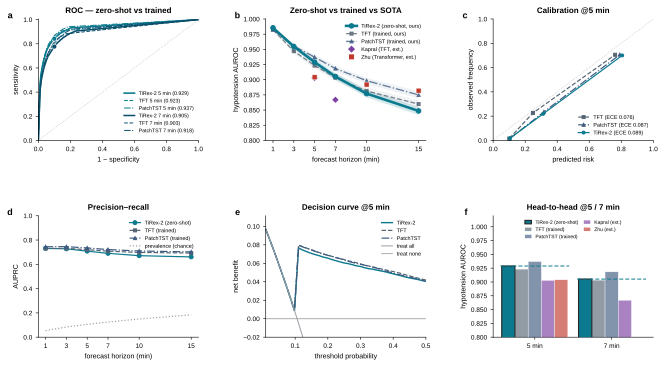
\includegraphics[width=\textwidth]{Fig4_hypotension_vs_sota.png}
\caption{\textbf{Impending-hypotension prediction versus supervised state of
the art on VitalDB.} Zero-shot TiRex-2 against task-trained TFT and PatchTST,
with external literature comparators (Kapral, Zhu) marked where reported.
(a)~ROC curves at 5 and 7~min (AUROC in parentheses).
(b)~Hypotension AUROC across horizons for TiRex-2 (zero-shot) versus trained
TFT and PatchTST, with Kapral (TFT) and Zhu (Transformer) external-VitalDB
literature values overlaid; shaded bands are case-clustered bootstrap 95\% CIs.
(c)~Reliability (calibration) curves at 5~min with expected calibration error
(ECE).
(d)~Precision--recall (AUPRC) across horizons, with prevalence as the chance
line.
(e)~Decision curve at 5~min: net benefit versus threshold probability for
each model against treat-all and treat-none.
(f)~Head-to-head AUROC at 5 and 7~min; dashed line marks the zero-shot
TiRex-2 level.
See Table~\ref{tab:matched} for values and Table~\ref{tab:stats} for paired
tests; Supplementary Fig.~\ref{fig:dca} extends the decision-curve analysis to
both cohorts at representative horizons (1, 5 and 15~min).}
\label{fig:sota}
\end{figure}

% ---------- Table 4 : Matched hypotension AUROC vs trained SOTA ----------
\begin{table}[ht]
\centering\footnotesize
\caption{\textbf{Matched hypotension AUROC on VitalDB: zero-shot TiRex-2 versus task-trained TFT and PatchTST} ($n=2{,}665$ subjects). Task-trained models scored by subject-level 5-fold out-of-fold cross-validation; TiRex-2 is inherently held out. M1 = with drug covariate, M0 = without; $\pm$SD is across the 5 folds; bracketed intervals are case-clustered bootstrap 95\% CIs. Bold marks the best model at each horizon. Kapral/Zhu columns are external literature references.}
\label{tab:matched}
\resizebox{\textwidth}{!}{%
\begin{tabular}{lccccccc}
\toprule
Horizon (min) & TiRex-2 zero-shot [95\% CI] & TFT M1 [95\% CI] & PatchTST M1 [95\% CI] & TFT M0 & PatchTST M0 & Kapral ext.\ AUROC \citep{Kapral2024} & Zhu ext.\ AUROC \citep{Zhu2026} \\
\midrule
1  & \textbf{0.986} [0.984, 0.987] & 0.982 [0.980, 0.985]\,$\pm$0.003 & 0.983 [0.980, 0.985]\,$\pm$0.002 & 0.984 & 0.982 & 0.960 & --- \\
3  & 0.955 [0.951, 0.958] & 0.947 [0.943, 0.951]\,$\pm$0.003 & \textbf{0.956} [0.952, 0.959]\,$\pm$0.005 & 0.945 & 0.947 & 0.945 & --- \\
5  & 0.929 [0.924, 0.934] & 0.923 [0.918, 0.929]\,$\pm$0.005 & \textbf{0.937} [0.933, 0.941]\,$\pm$0.005 & 0.913 & 0.920 & 0.903 & 0.897 \\
7  & 0.905 [0.900, 0.911] & 0.903 [0.898, 0.909]\,$\pm$0.004 & \textbf{0.918} [0.914, 0.923]\,$\pm$0.005 & 0.888 & 0.897 & 0.867 & --- \\
10 & 0.877 [0.871, 0.883] & 0.881 [0.876, 0.887]\,$\pm$0.004 & \textbf{0.898} [0.893, 0.903]\,$\pm$0.005 & 0.858 & 0.871 & --- & 0.862 \\
15 & 0.849 [0.842, 0.855] & 0.860 [0.854, 0.866]\,$\pm$0.003 & \textbf{0.875} [0.869, 0.881]\,$\pm$0.004 & 0.831 & 0.846 & --- & 0.822 \\
\bottomrule
\end{tabular}}
\end{table}

\subsection{The role of covariate-awareness}

TiRex-2 is the one foundation model in the panel that can condition on the
known future drug-infusion plan, so we asked how much this capability actually
contributes---rather than assuming it explains its lead---by comparing TiRex-2
with and without the covariate on identical windows. In transition windows at
7~min---where the infusion changes over the horizon and the covariate can
carry information---conditioning on the drug plan (effect-site concentration)
gave a small but significant improvement over the covariate-free
configuration: a $+1.15\%$ CRPS reduction (95\% CI $+0.84$ to $+1.47$,
$p<0.001$) for TiRex-2 (Fig.~\ref{fig:accuracy}; Table~\ref{tab:stats}). The
three univariate foundation models cannot use the covariate at all, so their
benefit is zero by construction.

Stratifying the benefit by window type sharpens the interpretation
(Supplementary Table~\ref{tab:covariate_split}). The covariate helped
\emph{only} when the infusion actually changed over the horizon: in
transition windows the CRPS reduction was positive and significant from
3~min onward (rising from $+0.41\%$ at 3~min to $+1.42\%$ at 10~min),
whereas in steady windows---where the plan does not change---it was
consistently small and negative at every horizon ($-0.47\%$ to $-0.67\%$).
A model reacting to the unfolding outcome rather than to the planned
intervention would gain in both strata; the benefit's confinement to
transition windows indicates the model is using genuinely informative
changes in the known-future plan, not leaking the outcome (Discussion).

The more informative signal is the contrast with the task-trained models on
the same windows: their dependence on the covariate is far larger (TFT
$+7.12\%$, PatchTST $+12.48\%$; all $p<0.001$, Table~\ref{tab:stats}). A model
trained on the task learns to lean heavily on the covariate channel, whereas
the zero-shot model already carries a strong general prior over
blood-pressure dynamics and gains comparatively little from the added signal.
In other words, covariate-awareness distinguishes the exemplar and its effect
is significant and correctly directed, but it is not the main reason TiRex-2
leads the zero-shot field---its base forecasting quality is
(Sec.~\ref{sec:zeroshot}). We therefore read this as a zero-shot foundation model able to
exploit the known future infusion, not as a claim that ``the drug covariate
helps,'' which is already established for trained models \citep{Kapral2024}.

\begin{figure}[t]
\centering
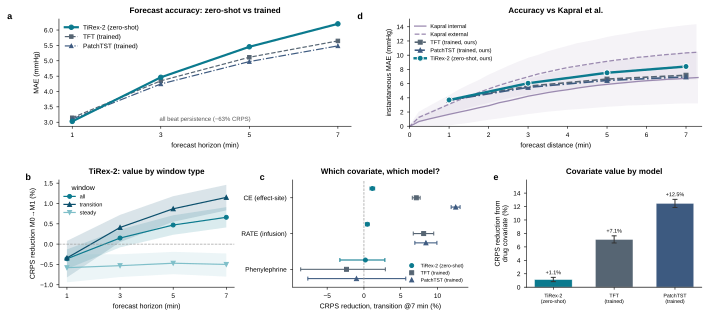
\includegraphics[width=\textwidth]{Fig2_accuracy_covariate.png}
\caption{\textbf{Forecast accuracy and the value of the known drug
covariate.} MAP forecast error and the CRPS benefit of conditioning on the
known-future drug-infusion covariate, for the covariate-aware exemplar
versus its covariate-free counterpart and the task-trained baselines. See
Table~\ref{tab:stats} for paired tests.}
\label{fig:accuracy}
\end{figure}

\subsection{Clinical translation and robustness}

Cast as an early-warning system at a fixed high-specificity operating point
($\geq$0.90), zero-shot TiRex-2 flagged impending hypotension with
clinically meaningful yield and lead time, remaining above the best
zero-shot comparator (Chronos-Bolt) while the task-trained baselines flagged more
events at every lead time and alarm budget (Fig.~\ref{fig:robust}a).
Sensitivity, positive and negative predictive value (PPV, NPV) and F1 across horizons (Supplementary Table~\ref{tab:opchar};
Fig.~\ref{fig:robust}b) followed the expected trade-off, with sensitivity
0.99$\rightarrow$0.64 and PPV 0.41$\rightarrow$0.60 from 1 to 15~min at
$\geq$0.90 specificity, and calibration, summarised by the expected calibration error (ECE), improving with horizon (0.122$\rightarrow$0.041). Discrimination was preserved under more severe
hypotension definitions (MAP\,$<$\,55, $<$\,50~mmHg, and MAP\,$<$\,65
sustained $\geq$5~min; Fig.~\ref{fig:robust}c). Performance was
equitable across prespecified clinical subgroups
(Fig.~\ref{fig:robust}d): at 5~min the 5-minute hypotension AUROC ranged
only from 0.916 to 0.939 around the overall 0.930 across sex, four age
bands (\,$<$50 to $\geq$80~y), ASA class (I--II vs III+), surgical
department and case-duration tertiles---a total spread of 0.023, with
every subgroup confidence interval overlapping the overall estimate and
no systematic deficit in any higher-risk stratum (older, higher-ASA, or
longer-duration cases). The zero-shot exemplar therefore
showed no evidence of differential performance across the demographic and
clinical axes recorded in VitalDB. This subgroup stability replicated on the
independent MOVER cohort (Fig.~\ref{fig:robust}d, lower panel), where the
5-minute AUROC ranged only from 0.885 to 0.906 across sex, age and
case-duration strata (spread 0.021, matching the 0.023 seen on VitalDB; ASA
class and surgical department are not recorded in MOVER). Reporting follows
the TRIPOD+AI
statement for prediction models using machine-learning methods
\citep{Collins2024}; a full item-by-item checklist is provided in
Supplementary Table~\ref{tab:tripod}.

The raw zero-shot risk scores were mildly under-dispersed (calibration slope
1.1--1.7, i.e.\ $>$1: predictions not extreme enough), reflecting the coarse
nine-level quantile grid of a training-free model, which compresses risk
toward the middle, rather than a discrimination deficit. A single post-hoc recalibration step
(isotonic regression fitted on each cohort's own disjoint development split and
applied to its held-out test split) reduced ECE to $\leq$0.012 at every horizon
on \emph{both} cohorts---correcting the largest raw values (0.122 at VitalDB
1~min; 0.123 at MOVER 15~min) entirely (Supplementary
Table~\ref{tab:calibration}). We emphasise that this recalibration was fitted
locally within each cohort: the VitalDB-fitted map did not transport reliably to MOVER
(external ECE 0.07--0.16, worse than raw at the 5- and 15-min horizons),
because MOVER's 2--3$\times$ higher prevalence shifts the calibration
intercept. Discrimination
(AUROC) is therefore label-free and portable, but \emph{calibration} correction
requires a one-off labelled subset from the target cohort---a modest
requirement, but not a zero-label one. This is, in effect, a favourable
division of labour along the label axis: discrimination is obtained zero-shot,
while a light \emph{few-shot} step---a small labelled sample from the deployment
site, used only to fit a monotone recalibration map and leaving the model
weights untouched---suffices to make the risk scores locally reliable. Site
adaptation here is a calibration exercise on tens of labelled cases, not a
retraining exercise on a large site-specific cohort. After recalibration, decision-curve analysis
showed net benefit exceeding both default strategies---treat-all and
treat-none---across essentially the whole range of clinically plausible alarm
thresholds (2--35\% risk) on both cohorts (Supplementary Fig.~\ref{fig:dca}):
on VitalDB across the full threshold range (100\%) at 1 and 5~min and 91\% at 15~min (e.g.\
at 5~min and a 10\% threshold, net benefit 0.081 vs 0.007 for treat-all and 0
for treat-none), and on MOVER over 100\%/88\%/68\% of thresholds at
1/5/15~min, the narrowing at 15~min reflecting MOVER's 41\% event prevalence,
which raises the treat-all reference. The recalibrated forecasts therefore
translate into positive decision value, not discrimination alone.

\begin{figure}[t]
\centering
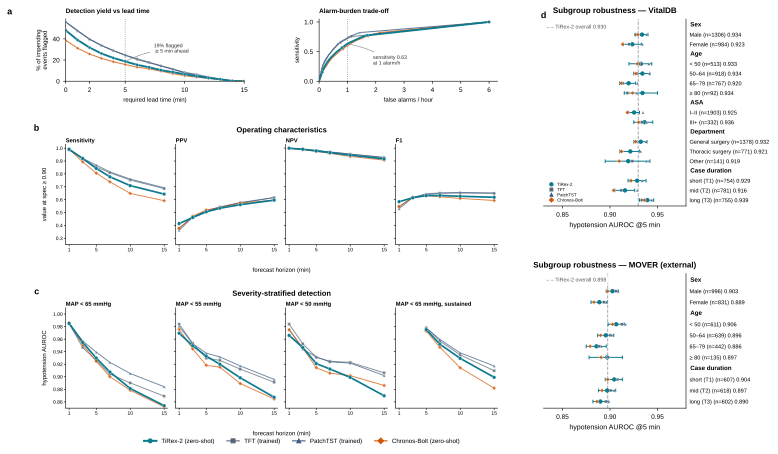
\includegraphics[width=\textwidth]{Fig5_clinical_robustness.png}
\caption{\textbf{Clinical translation and robustness.}
(a)~Early-warning yield versus lead time at fixed specificity.
(b)~Operating characteristics across horizons.
(c)~Discrimination under more severe hypotension definitions.
(d)~Subgroup stability of 5-minute hypotension AUROC across prespecified
clinical strata, for VitalDB (top) and the independent MOVER cohort
(bottom); points are subgroup AUROC with case-clustered bootstrap 95\%
confidence intervals, the dashed line the overall estimate, and the three
comparator models overlaid. ASA class and surgical department are recorded
only in VitalDB.}
\label{fig:robust}
\end{figure}

\subsection{External validation and cross-dataset transfer}

The identical zero-shot model applied to the independent MOVER cohort held
AUROC\,$\geq$\,0.85 across all horizons despite the 2--3$\times$ higher
hypotension prevalence and the 60~s sampling cadence: 0.947 (95\% CI
0.943--0.951) at 1~min to 0.853 (0.847--0.859) at 15~min
(Table~\ref{tab:external}). Forecast error remained close to the
development cohort (external MAE 3.74~mmHg at 1~min to 7.73~mmHg at 15~min).
At a fixed specificity of 0.90, the higher external prevalence translated
into substantially higher positive predictive value than on the development
cohort---PPV rose from 0.65 at 1~min (16.7\% prevalence) to 0.82 at 15~min
(41.4\% prevalence), with AUPRC 0.80--0.83 across horizons
(Supplementary Table~\ref{tab:mover_opchar}).

These external AUROC values must, however, be read against the naive
persistence floor, which is exceptionally high on MOVER's 60~s grid
(Supplementary Table~\ref{tab:naive}). At the shortest horizons the
last-observed-MAP alarm alone reached AUROC 0.997/0.952/0.918 at 1/3/5~min,
\emph{above} every learned model---zero-shot TiRex-2 (0.948/0.917/0.898) and
the in-domain-trained TFT and PatchTST (both $\approx$0.945/0.920/0.905)
alike (Supplementary Table~\ref{tab:naive_learned}). The learned models
overtook persistence only from about 10~min onward (e.g.\ TiRex-2 $+0.003$ at
10~min, $+0.010$ at 15~min). In other words, on the external cohort at high
cadence the short-horizon task is very largely solved by autocorrelation, so
an AUROC of $\geq$0.85 at 1--5~min reflects the ease of the label there
rather than any distinctive skill of the learned models; the value of a
forecaster---foundation or supervised---is concentrated at the longer
horizons, where persistence degrades and the learned models separate from it.
This mirrors the caution raised against earlier hypotension-warning systems,
that discrimination can look strong while adding little over a simple
threshold alarm~\citep{Enevoldsen2022,Vistisen2024}; we report the floor
explicitly so the external result is not over-read.
The external-cohort foundation-model benchmark reproduced the
development-cohort ranking---TiRex-2 led Chronos-Bolt, TimesFM-2.5 and
Moirai-1.1-R on AUROC at every horizon
(Table~\ref{tab:zeroshot_mover}; Supplementary Fig.~\ref{fig:zeroshot_mover})---so the
paradigm result---that TiRex-2 is the strongest zero-shot forecaster and
holds clinically useful discrimination---replicates on the independent
cohort. We did not repeat the covariate ablation on MOVER, which carries
only an infusion-rate covariate rather than the effect-site concentration
used on VitalDB; the external evidence therefore speaks to the paradigm and
the foundation-model ranking, not to the covariate-awareness effect
specifically (Limitations).

In the cross-dataset transfer analysis (covariate-free, both cohorts
harmonised to 60~s cadence; Supplementary Table~\ref{tab:transfer}; Fig.~\ref{fig:transfer}),
zero-shot TiRex-2 was the strongest model on VitalDB at every horizon and,
on MOVER, matched the models trained in-domain on MOVER (5-fold out-of-fold)
while beating both baselines transferred from VitalDB. For example, on MOVER
at 5~min TiRex-2 reached 0.899, against in-domain TFT 0.903 and PatchTST
0.901 but transferred TFT 0.895 and transferred PatchTST 0.895. On
case-clustered bootstrap paired tests (Supplementary Table~\ref{tab:transfer}),
zero-shot TiRex-2's advantage over the VitalDB-transferred baselines was
significant at the shortest and longest horizons (e.g.\ $+0.007$ vs
transferred TFT at both 1 and 15~min, $p<0.001$), whereas its gap to the
in-domain-trained models was small and mostly within confidence intervals
(all $|\Delta\text{AUROC}|\leq0.012$). A single pretrained model, applied
without any labels, was competitive with cohort-specific supervised training
and superior to supervised transfer---the portability argument for the
paradigm, demonstrated directly.

\begin{figure}[t]
\centering
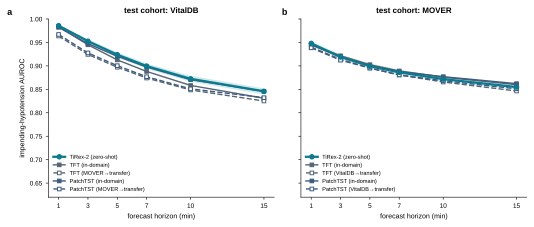
\includegraphics[width=\textwidth]{Fig6_transfer.png}
\caption{\textbf{Cross-dataset transfer and external validation.} Zero-shot
TiRex-2 (training-free anchor) versus TFT and PatchTST trained in-domain
(solid) and transferred across cohorts (dashed), on VitalDB and MOVER test
sets harmonised to 60~s cadence. See Supplementary Table~\ref{tab:transfer}.}
\label{fig:transfer}
\end{figure}

% ---------- Table 8 : External validation (VitalDB vs MOVER) ----------
\begin{table}[ht]
\centering\footnotesize
\caption{\textbf{External validation: zero-shot TiRex-2 on VitalDB versus the independent MOVER cohort.} MOVER uses an invasive arterial MAP source at 60 s cadence with 2--3$\times$ higher hypotension prevalence. AUROC holds $\geq$0.85 across all horizons on MOVER.}
\label{tab:external}
\resizebox{\textwidth}{!}{%
\begin{tabular}{lcccccccc}
\toprule
 & \multicolumn{4}{c}{VitalDB (development)} & \multicolumn{4}{c}{MOVER (external)} \\
\cmidrule(lr){2-5}\cmidrule(lr){6-9}
Horizon (min) & AUROC [95\% CI] & CRPS & MAE & prev.\% & AUROC [95\% CI] & CRPS & MAE & prev.\% \\
\midrule
1  & 0.985 [0.984, 0.987] & 1.251 & 3.03 & 5.4  & 0.947 [0.943, 0.951] & 1.540 & 3.74 & 16.7 \\
3  & 0.955 [0.951, 0.958] & 1.827 & 4.46 & 8.4  & 0.917 [0.912, 0.921] & 2.065 & 5.05 & 23.3 \\
5  & 0.929 [0.924, 0.934] & 2.221 & 5.46 & 10.6 & 0.898 [0.893, 0.903] & 2.387 & 5.86 & 28.1 \\
7  & 0.905 [0.900, 0.911] & 2.515 & 6.20 & 12.5 & 0.885 [0.880, 0.890] & 2.615 & 6.44 & 31.7 \\
10 & 0.877 [0.871, 0.883] & 2.839 & 7.01 & 15.0 & 0.870 [0.864, 0.875] & 2.861 & 7.05 & 36.1 \\
15 & 0.849 [0.842, 0.855] & 3.213 & 7.95 & 18.4 & 0.853 [0.847, 0.859] & 3.140 & 7.73 & 41.4 \\
\bottomrule
\end{tabular}}
\end{table}

\subsection{What the zero-shot representations encode}

A natural question is \emph{why} a model that never saw this task can rival one
trained on it---and, for a prospective user, whether the risk these models
produce can be read directly off an internal representation or only through
their calibrated forecasts. We probed the internal representations of all six
models on an identical 4{,}000-window subsample of each cohort, taking each
model's pooled penultimate-layer activation as a per-window representation and
asking what it linearly encodes (Methods). Three analyses converge on a single,
initially counter-intuitive answer with a direct practical corollary:
\emph{zero-shot forecasting skill and linear representational structure are
decoupled}---so these models must be used as forecasters, through their
multi-horizon predictions, not as feature extractors from which hypotension
risk is read off linearly.

First, the clinical label is only weakly and diffusely embedded in the zero-shot
representations. Projected with UMAP \citep{McInnes2018} and coloured by impending hypotension
(Supplementary Fig.~\ref{fig:umap_vitaldb}), the label appears as a gradient
rather than as separated clusters, and a subject-grouped linear probe quantifies
its strength (Supplementary Table~\ref{tab:probe_hypo}). The task-trained models
expose the label almost perfectly (TFT AUROC 0.97 at 1~min, 0.89 at 15~min)
because their loss was defined to do so; among the zero-shot models the
univariate Chronos-Bolt and Moirai carry partial structure (AUROC $\approx$
0.66--0.71) while TiRex-2 and TimesFM-2.5 sit at chance (0.44--0.53). The
ordering is stable across horizons and---most tellingly---inverts against
forecasting skill: TiRex-2, the strongest forecaster, has the \emph{least}
task-separable representation.

Second, the same decoupling holds for the continuous quantity a forecaster
should encode. A ridge probe for mean arterial pressure itself---current level,
near-future mean and minimum, and slope---is linearly successful only for the
task-trained TFT ($R^2\approx0.8$--0.96 for current and near-future level),
while the zero-shot models are weak to negative, TiRex-2 included
($R^2\approx-0.08$, no better than the mean; Supplementary
Table~\ref{tab:probe_traj}). A forecaster's skill therefore resides in its full
encoder$\rightarrow$decoder mapping conditioned on the known-future covariates,
not in a linearly-decodable summary of its pooled penultimate state, which
discards the temporal detail the forecast head uses.

Third, where the representations \emph{do} show strong discrete structure, it is
not clinical. Several models split into separated groups in the UMAP, but a
characterisation of that split (Supplementary Table~\ref{tab:cluster_char})
shows it never encodes the outcome: the strongly bimodal zero-shot models
(TimesFM-2.5, TiRex-2) split on embedding-activation magnitude (an internal
scale artifact), the task-trained models split near-purely by case on surgical
department, and Chronos-Bolt/Moirai are effectively unimodal. Consistent with
this, cross-model representational similarity (linear CKA, Supplementary
Fig.~\ref{fig:rsa_cka}) is near zero between the zero-shot and task-trained
families and even among the zero-shot models---the only substantial similarities
are within family (Chronos-Bolt$\leftrightarrow$Moirai, TFT$\leftrightarrow$PatchTST).
The four foundation models reach comparable forecasting performance through
distinct, non-aligned internal geometries. All three findings replicate on the
external MOVER cohort (Supplementary Fig.~\ref{fig:umap_mover}; Supplementary
Tables~\ref{tab:probe_hypo}--\ref{tab:cluster_char}). The practical implication
is that these are forecasters, not patient-state classifiers: their value is
realised through calibrated multi-horizon prediction (\S2.4), not through a
representation from which risk can be read off linearly.

\section{Discussion}

Across two cohorts, a general-purpose time-series foundation model applied
zero-shot was competitive with task-trained models for intraoperative MAP
forecasting and impending-hypotension prediction: on par with TFT at the
short-to-mid horizons though behind the stronger PatchTST beyond 5~min, and
ahead of every other zero-shot foundation model, with the ranking reproduced
on the external MOVER cohort. We stress the scope of the covariate-awareness
claim: only TiRex-2 among the models tested is covariate-aware, so this is a
statement about the best exemplar, not about foundation models as a class,
three-quarters of which (the univariate comparators) cannot ingest a
covariate at all.

\paragraph{Relation to the state of the art.} Our work is positioned
directly against two recent task-trained models. Kapral et al.\ forecast the
MAP trajectory with a TFT conditioned on medication as observed history, and
identified---but by construction could not close---the gap we address: their
model ``cannot and should not'' use interventions administered after the
prediction origin, and its external overestimation of hypotension reflects a
model ``not anticipating future medical interventions'' \citep{Kapral2024}.
By feeding the known future infusion trajectory over the forecast horizon to
a zero-shot model, we operate in exactly the regime they name as out of
reach. Zhu et al.\ deliberately omit medication, arguing vital signs
implicitly encode drug effects \citep{Zhu2026}; our covariate ablation is
the first direct empirical test of that assumption in this setting, and the
small-but-significant benefit of the future-known covariate indicates the
assumption is not exactly true---an explicit intervention signal adds
information beyond what the vital-sign trajectory carries. Crucially, our
novel claim is not that drug data helps a MAP forecast---Kapral established
that for trained, past-covariate models---but the \emph{conjunction} of
zero-shot operation and known-future conditioning, quantified as a paired,
per-horizon, CI-bearing comparison.

\paragraph{Why the paradigm matters clinically.} Both comparator models require training
on large, site-specific labelled cohorts (73{,}009 cases for Kapral et al.\
\citep{Kapral2024} and 319{,}699 for Zhu et al.\ \citep{Zhu2026}). The
central practical advantage we demonstrate is portability: one pretrained
model, no task-specific labels, competitive with cohort-specific supervised
training and superior to supervised transfer across a real distribution
shift (different cadence, covariate availability, population, and
2--3$\times$ hypotension prevalence). For institutions without the data
scale or labelling infrastructure to train a bespoke model, a training-free
approach that reaches supervised-comparable discrimination at urgent
horizons is an attractive off-the-shelf option. This portability does not
come at a prohibitive compute cost: at 82.5~M parameters TiRex-2 is the
smallest of the four foundation models, all six models run inference within
$\approx$1.6~GB of GPU memory, and per-window latency is well below the 15~s
acquisition cadence (Supplementary Table~\ref{tab:compute_footprint}), so the
zero-shot approach is deployable on commodity hardware in real time. Unlike
the HPI, our approach uses low-resolution numeric vital signs with no
arterial waveform and no proprietary index
\citep{Hatib2018,Enevoldsen2022,Vistisen2024}, and unlike both trained
comparators it needs no local training run before deployment.

\paragraph{Where task-trained models remain ahead, and where a naive alarm
does.} The comparison must be read on two axes: against the trained baselines
and against a naive persistence floor. Of the two trained baselines, TiRex-2
was on par with or above TFT across 1--7~min but was outperformed by the stronger PatchTST from
5~min onward (5~min AUROC 0.929 vs 0.937, $p<0.001$; 7~min 0.905 vs 0.918,
$p<0.001$; 15~min 0.849 vs 0.875), so the ``match against task-trained
models'' holds specifically against TFT at short horizons, not against the
best supervised model across the range. On continuous accuracy the trained
models were also lower-error beyond 1~min (15~min MAE 7.95 vs 6.82~mmHg for
TFT and 6.68 for PatchTST; CRPS 3.213 vs 2.656 for PatchTST). Against the
naive floor, the picture is horizon- and cadence-dependent: on VitalDB
(15~s) persistence is best only at 1~min and is cleared by the strongest
learned model at each horizon from 3~min onward (TiRex-2 and PatchTST at
3~min; all three by 7~min), whereas on MOVER (60~s) persistence exceeds all
learned models through 5~min and is overtaken only from 10~min (Supplementary
Table~\ref{tab:naive_learned}). The honest reading is therefore narrower than
a blanket ``competitive at urgent horizons'': at the very shortest horizons
the task is close to solved by autocorrelation, so no model---zero-shot or
supervised---adds much; TiRex-2's genuinely favourable regime is the middle
horizons (roughly 3--7~min on VitalDB, where it clears the naive floor and
matches TFT), while task-trained models specialise best at the longest
horizons. What the zero-shot paradigm adds is not a uniform accuracy
advantage but portability---supervised-comparable discrimination with no
task-specific labels or training run---which is most valuable exactly where
bespoke models are hardest to build.

\paragraph{Limitations.} First, the known-future infusion trajectory we
condition on is the drug regimen the clinician actually delivered, recorded
retrospectively---an optimistic upper bound relative to deployment, where
the future drug plan is not known exactly in advance. This is the mirror
image of Kapral's reactive-intervention miscalibration: their trained model
overestimates hypotension because it cannot anticipate interventions,
whereas our model benefits because it is given them. Two observations bound
how large this advantage can be. The covariate benefit is confined to
transition windows and is absent (indeed slightly negative) in steady
windows (Supplementary Table~\ref{tab:covariate_split}); this is consistent
with the model using informative changes in the planned infusion, though we
note it is not decisive, because a clinician who lowers the infusion in
response to a falling MAP produces an infusion change that also lives in the
transition stratum---so reactive titration cannot be fully excluded by this
split alone, and the definitive test is the deferred planned-versus-realised
infusion analysis. What the split does establish is that the effect is not a
blanket steady-state gain. And the benefit is small in absolute terms
($\leq1.4\%$ CRPS reduction), so even if the planned infusion in deployment
were less informative than the realised one, the headline paradigm
result---which holds in the covariate-free configuration---would be largely
unaffected. Prospective evaluation with the \emph{planned} rather
than realised infusion remains the necessary next step to close this gap
directly. Second, the covariate here is the anaesthetic infusion (remifentanil
$\pm$ propofol); continuous vasopressor-infusion channels are near-absent in
VitalDB, and bolus drugs are unrecorded \citep{Kapral2024}, so the
intervention$\rightarrow$response relationship we model is anaesthetic-induced
blood-pressure change. Third, both cohorts are retrospective; VitalDB is
single-centre and selected for infusion cases. Both cohorts also derive MAP
from an \emph{invasive arterial line} in the operating room; we have not
demonstrated portability to non-invasive (oscillometric) blood pressure or to
other care settings---the intensive care unit, the ward, the emergency
department or the post-anaesthesia care unit---where signal cadence, noise,
artefact profile and hypotension epidemiology all differ, and where the
availability and meaning of the drug-infusion covariate would change. Claims of
portability here are therefore between two intraoperative arterial-line cohorts,
not across monitoring modalities or settings. Fourth, the foundation models
are pretrained on large, undisclosed time-series corpora, and we cannot rule
out that public physiological datasets---including VitalDB, which is openly
downloadable and has appeared in prior time-series collections---were seen
during pretraining. Two considerations bound this concern but do not
eliminate it. The task labels (hypotension events) and the forecasting
protocol are ours and were never used to train the models, so any exposure
would be to the raw MAP series, not to the supervised target; and the ranking
reproduces on MOVER, an access-controlled cohort released after several of
these models' pretraining windows and far less likely to have been ingested.
Even so, a fully contamination-free evaluation would require held-out data
postdating every model's pretraining cut-off, which the model providers do
not disclose precisely; we therefore report possible pretraining exposure as
an unquantified but bounded risk rather than a resolved non-issue. Fifth,
hypotension labels are defined at each cohort's native cadence (15~s on
VitalDB, 60~s on MOVER); the coarser MOVER grid can miss brief sub-minute
excursions and merge closely spaced events, so prevalence and operating
characteristics are not strictly cadence-matched across cohorts and the two
are reported stratified rather than pooled. Sixth, the covariate
benefit, while significant, is small for the zero-shot exemplar, and the
paradigm's advantage is concentrated at short horizons. Finally, this is a
research analysis, not a medical device; the secondary early-warning task
should be reported against TRIPOD-AI when carried toward clinical
translation \citep{Collins2024}, and prospective, real-time trials---as both
comparator studies also emphasise---are required before clinical implementation.

\paragraph{Conclusion.} Zero-shot, covariate-aware time-series foundation
models are a competitive and portable paradigm for intraoperative
hypotension prediction, matching task-trained TFT at short-to-mid horizons across two cohorts
without any task-specific training, above a strong short-horizon persistence
floor that only the longer horizons clear.
Conditioning on the known future intervention plan is the feature that
distinguishes the leading exemplar. These results motivate prospective
evaluation using planned drug regimens and, in the longer term, the use of
such models as training-free components of hemodynamic decision support.

\section{Methods}

\subsection{Datasets and cohort curation}

\paragraph{VitalDB (development).} VitalDB is an open high-resolution
intraoperative vital-signs database from Seoul National University Hospital
\citep{Lee2022,VitalDBPhysioNet2022}. We built the development cohort from
locally materialised \texttt{.vital} files using the \texttt{vitaldb}
package. Each candidate case passed through an inclusion cascade, recorded as
a case-flow funnel (Fig.~\ref{fig:design}b): a header check for the required
tracks; presence of an invasive mean arterial pressure signal
(\texttt{Solar8000/\allowbreak ART\_MBP}); presence of a remifentanil infusion
(\texttt{Orchestra/\allowbreak RFTN20\_CE} and \texttt{RFTN20\_RATE}); anaesthesia
duration $\geq$60~min (leaving room for a 30-min context, the longest
horizon and multiple rolling origins); MAP coverage $\geq$0.60 of finite
samples over the anaesthesia window; remifentanil effect-site coverage
$\geq$0.50; and an \emph{infusion-fidelity} gate requiring a genuinely active
infusion (maximum effect-site concentration $>$0.5~ng\,mL$^{-1}$), so that
the drug covariate carries real signal rather than a flat zero trace. Cases
were excluded, in order, for an unreadable header, missing arterial MAP,
missing remifentanil, load failure, insufficient duration, low MAP coverage,
low remifentanil coverage, or an inactive infusion. The final development
cohort comprised 2{,}708 cases contributing 47{,}642 forecast windows
(Table~\ref{tab:cohort}). These 2{,}708 cases correspond to 2{,}665 unique
subjects (some patients contributed more than one operation); all splits,
cross-validation folds and bootstrap resampling were defined at the subject
level, so the matched analyses report $n=2{,}665$ subjects.

\paragraph{MOVER (external validation).} The Medical Informatics Operating
Room Vitals and Events Repository (MOVER) is a public multicentre
operating-room database \citep{Samad2023,MOVERUCI2023}. A dataset-agnostic
loader maps the MOVER source-information-system columns onto the same
canonical channel names used for VitalDB (invasive arterial MAP as the
target; derived propofol$+$remifentanil infusion rate as the covariate; heart
rate, peripheral oxygen saturation and central venous pressure as past
covariates), so the entire downstream pipeline runs unchanged. A patient was
included with $\geq$30~min of invasive arterial MAP within the
operating-room window and at least one whitelisted continuous infusion. The
external cohort comprised 1{,}827 cases. Both cohorts use an invasive arterial MAP source; the two differ in
sampling cadence (15 vs 60~s),
available covariates (effect-site concentration and rate vs rate only) and
hypotension prevalence (2--3$\times$ higher on MOVER), and were analysed
strictly stratified and never pooled.

\subsection{Signal preprocessing and windowing}

VitalDB signals were loaded on a native $\approx$0.5~Hz (5~s) grid and
downsampled to a 15~s grid at load time by block aggregation (median for the
MAP target; last-value hold for the step-like drug channels); MOVER signals
are natively 60~s and were not upsampled. Recordings were trimmed to the
anaesthesia window. Physiologically implausible values were set to missing
using fixed plausibility ranges (MAP 20--220~mmHg; heart rate 20--220~min
$^{-1}$; oxygen saturation 50--100\%; central venous pressure
$-5$ to 40~mmHg), which removes arterial-line zeroing, disconnection and
transducer artefacts; drug channels had negative values clipped to zero. The
MAP target was additionally despiked by flagging samples deviating more than
25~mmHg from a 35~s rolling median (window of 7 samples at 5~s), which
removes fast-flush and transient arterial-line spikes the range mask misses.
Missing values were left as such and handled natively by the forecasters
(TiRex-2 masks non-finite inputs; the supervised baselines received
finite-filled tensors with the target normalised per window).

From each case we extracted rolling-origin windows: a 30-min context
predicting the MAP trajectory over the horizon, with origins spaced 5~min
apart, a 15-min warm-up before the first origin, and up to 20 origins per
case. A window was retained when at least 50\% of both its context and its
horizon target samples were finite and, for covariate-conditioned
conditions, the future covariate was fully observed over the horizon. Windows
were tagged as \emph{transition} or \emph{steady} according to whether the
drug effect-site concentration changed over the horizon, so the covariate
effect could be assessed where it is mechanistically expected to matter.

\subsection{Forecasting task and covariate conditions}

For every rolling origin we forecast MAP at horizons of 1, 3, 5, 7, 10 and
15~min and predicted impending hypotension, defined as MAP\,$<$\,65~mmHg
occurring within the horizon (sustained for $\geq$1~min). The known-future
covariate was the planned drug-infusion trajectory---remifentanil
$\pm$ propofol effect-site concentration on VitalDB, infusion rate on
MOVER---supplied over the entire context-plus-horizon span. We evaluated four
covariate conditions per window: M1 (target, past covariates and the
known-future drug covariate), M0 (identical but with the future covariate
withheld), and two target-only arms (with and without the future covariate,
omitting the past covariates) used to test whether the past vital-sign
trajectory already encodes the drug effect. The covariate benefit is the
fractional CRPS reduction from M0 to M1.

\subsection{Models}

\paragraph{Zero-shot foundation models.} TiRex-2 is a multivariate,
streaming-capable zero-shot forecaster built on a bidirectional xLSTM
(extended long short-term memory) stack in which the reverse pathway is
restricted to known covariates, allowing it to condition on both past and
known-future inputs \citep{Auer2025,Podest2026}. It emits nine quantile
levels (0.1--0.9); the median is the point forecast and the full set of
quantiles is the probabilistic forecast used for CRPS and for hypotension
risk (the probability mass below 65~mmHg). Chronos-Bolt (a T5
encoder--decoder that outputs multi-step quantiles directly \citep{Ansari2024}),
TimesFM-2.5 (a decoder-only patched forecaster with a continuous quantile
head \citep{Das2024}) and Moirai-1.1-R (a masked-encoder any-variate model
whose sample forecasts we reduced to empirical quantiles \citep{Woo2024}) are
univariate: each produces one forecast per window that is reused for the M1
and M0 columns, so their covariate benefit is zero by construction. No
foundation model was trained or fine-tuned at any point; all were run from
their released pretrained checkpoints (Model availability). Every foundation
model self-normalises, so it received the raw MAP context directly, and all
were scored on identical windows with the same metric code as the supervised
baselines.

\paragraph{Task-trained baselines.} We trained two supervised baselines from
scratch as covariate-aware, quantile-forecasting references. The Temporal
Fusion Transformer (TFT) \citep{Lim2021} combines per-timestep variable
selection, gated residual networks, an LSTM encoder--decoder split at the
forecast origin (so known-future covariates enter the decoder) and
interpretable multi-head self-attention with a causal mask, followed by a
quantile head (hidden size 64, 4 attention heads, dropout 0.1). PatchTST
\citep{Nie2023} lays every channel---target, past covariates and known-future
drug covariates---over the full context-plus-horizon span (past channels
zero-padded across the horizon, future covariates carrying their known values
throughout), splits each into overlapping patches of length 16 with stride 8,
patch-embeds them, passes them through a shared 3-layer Transformer encoder
(model dimension 96, 4 heads) and emits the target's horizon quantiles from a
joint head over all channels' patch tokens. In both models the M0 arm zeroes
the future-covariate channels upstream, leaving architecture and training
identical.

Both baselines were trained by minimising the pinball (quantile) loss over
the nine quantile levels $\mathcal{Q}=\{0.1,\dots,0.9\}$, which is a discrete
approximation of the CRPS. For a target $y$, a predicted quantile $\hat y_q$
at level $q$ and a validity mask $m$,
\begin{equation}
\mathcal{L} = \frac{\sum_{t}\, m_t \, \frac{1}{|\mathcal{Q}|}\sum_{q\in\mathcal{Q}}
\max\!\big(q\,(y_t-\hat y_{q,t}),\,(q-1)\,(y_t-\hat y_{q,t})\big)}
{\sum_{t} m_t}\, .
\end{equation}
Optimisation used Adam (learning rate $10^{-3}$, weight decay $10^{-5}$) with
learning-rate reduction on plateau (factor 0.5, patience 3 epochs), gradient
clipping at 1.0, batch size 256, up to 60 epochs with early stopping
(patience 8 epochs on the validation loss), and up to 20 rolling origins per
case.

\subsection{Evaluation protocol and cross-dataset transfer}

Splits were defined at the subject level so that no subject appeared in more
than one partition. For the head-to-head against the zero-shot model, the
supervised baselines were evaluated by subject-level 5-fold cross-validation
with out-of-fold prediction: subjects were partitioned into 5 folds (seeded,
round-robin over a shuffled subject list), and each fold was predicted by a
model trained on the other folds (with the next fold held out for
validation), so that every case received a prediction from a model that never
saw it in training. This makes the supervised comparison against the
inherently held-out zero-shot forecaster apples-to-apples: all models are
scored on identical, unseen windows. Per-fold learning curves confirmed
convergence without overfitting on both cohorts (Supplementary
Fig.~\ref{fig:training_curves}).

For cross-dataset transfer (Fig.~\ref{fig:transfer}; Supplementary
Table~\ref{tab:transfer}), each baseline was additionally trained on the
entire source cohort (with a 10\% subject-level validation holdout) and
applied to the other cohort using the source normalisation; ``in-domain''
performance is the held-out 5-fold out-of-fold result and ``transfer'' is the
all-cases checkpoint applied across cohorts. Because the two cohorts differ
in cadence and covariate units, transfer was run covariate-free (M0) with
both cohorts harmonised to a 60~s cadence and matched channel counts.

Probabilistic forecasts were scored by the continuous ranked probability
score (CRPS) and by mean absolute error (MAE) and root-mean-square error
(RMSE) on the predictive median. Impending-hypotension discrimination was
scored by AUROC and by the area under the precision--recall curve (AUPRC),
with calibration summarised by the ECE and by operating characteristics (sensitivity,
PPV, NPV, F1) at a fixed specificity $\geq$0.90. All aggregation used
case-clustered inference to account for repeated windows within a case; 95\%
confidence intervals and paired significance tests used a case-clustered
bootstrap (2{,}000 resamples, cases resampled with replacement, each
comparison paired on identical windows and differenced within resample).
The evaluation protocol (horizons, context, origin stride, warm-up,
hypotension threshold and bootstrap settings) was fixed in a configuration
file and applied identically to every model and both cohorts.

\subsection{Hardware and implementation}

The supervised baselines and the covariate ablation were run on NVIDIA A100
GPUs on the Medical University of Vienna high-performance computing cluster;
foundation-model inference is zero-shot and was executed from released
checkpoints. Models and the evaluation pipeline were implemented in PyTorch.
All runs were seeded, and the full configuration, cohort builders, dataset
loaders and evaluation code are released as described under Code
availability. To characterise deployment cost, we measured each model's
parameter count, one-off load time, per-window inference latency (and
throughput) and peak GPU memory on a single A100, timing the identical
forecast calls used to produce the results over a fixed 512-window sample
(Supplementary Table~\ref{tab:compute_footprint}); no model was retrained for
this measurement.

\subsection{External literature comparators}

Kapral et al.\ \citep{Kapral2024} and Zhu et al.\ \citep{Zhu2026} are
reported as external reference points from their publications, not
re-executed. Their published external-VitalDB AUROC values were extracted
from the main text of the respective papers and appear alongside ours in
Tables~\ref{tab:classification} and~\ref{tab:matched} and in
Fig.~\ref{fig:sota}, clearly marked as literature values. Where a value was
reported only graphically---specifically the mean absolute error curve of
Kapral et al.---it was recovered from the published figure using a
plot-digitization tool \citep{WebPlotDigitizer}. These are
\emph{contextual} comparisons, not head-to-head benchmarks: the two studies
differ from ours in preprocessing, patient selection, outcome definition,
cohort construction and evaluation protocol, so the absolute values are not
strictly commensurable and should be read as external points of reference
that situate our results within the reported literature, not as a controlled
comparison on identical data.

\subsection{Representation analysis}

To characterise what each model's internal representation encodes, we extracted
one representation vector per forecast window from the model's penultimate stage,
pooled over the sequence to a single vector. For the zero-shot models this was
the final encoder hidden state, taken from the documented embedding interface
where available (Chronos-Bolt) and otherwise from a fixed, pre-registered module
selected from the model's architecture---the encoder-stack output norm for
TiRex-2 (dimension 512), the last transformer block for TimesFM-2.5 (1{,}280),
and the encoder output norm for Moirai-1.1-R (1{,}024); for TimesFM-2.5 the
context-encoding pass was used, which is horizon-independent. For the two
task-trained baselines the representation was the penultimate layer before the
forecast head (TFT position-wise gated residual output, mean-pooled over the
horizon; PatchTST post-encoder norm, mean-pooled over patches and channels; both
dimension 64). All six models were run on the identical seeded 4{,}000-window
subsample per cohort (stratified by window stratum and 5-min hypotension label),
so the resulting representations are row-aligned across models. Linear
separability of impending hypotension was assessed with an $L_2$-regularised
logistic probe (scikit-learn \citep{Pedregosa2011}) under 5-fold subject-grouped cross-validation (no subject shared
between train and test), reported as AUROC and AUPRC; continuous MAP quantities
were probed analogously with ridge regression ($R^2$). Discrete structure was
summarised by a 2-means split of each representation, its silhouette, and its
association with candidate variables (adjusted mutual information for categorical
variables, split AUROC for continuous ones, and case purity). Cross-model
representational similarity used linear centred kernel alignment
\citep{Kornblith2019}, which is invariant to the differing representation
dimensions. No representation was fine-tuned; probes were fitted only for this
analysis and play no part in the forecasting or hypotension results.

\subsection{Reproducibility}

All figures, tables and statistics were generated by a deterministic pipeline
(seeded runs, a configuration-file evaluation protocol, and per-window
forecasts and per-case metrics saved to disk) and assembled into a single
results bundle. Upon acceptance, the complete pipeline---together with the
curated training/validation/test splits and cohort manifests---will be
deposited in a public Zenodo archive with a citable DOI, providing a frozen,
versioned snapshot of the exact code and derived data used here (subject to
the source datasets' data-use terms, as detailed under Code availability).
Ongoing development, issue tracking and any post-publication updates will be
maintained in a companion GitHub repository, linked from the Zenodo record,
so that the archived snapshot remains citable while the living codebase
continues to be supported.

\section*{Data availability}
VitalDB is openly available at \url{https://vitaldb.net} and via PhysioNet
\citep{VitalDBPhysioNet2022}. MOVER is a public-access operating-room
database, available from the UCI Machine Learning Repository
\citep{Samad2023,MOVERUCI2023}. The curated cohort manifests and
train/validation/test splits derived from these sources are released as
described under Code availability.

\section*{Code availability}
The full analysis and figure-generation pipeline, evaluation configurations,
cohort builders and dataset loaders, together with the curated
training/validation/test splits and cohort manifests used in this study,
will be released upon acceptance as a frozen, versioned snapshot in a public
Zenodo archive with a citable DOI, with ongoing development maintained in a
companion GitHub repository linked from the Zenodo record. Release is to the
extent permitted by the source datasets' data-use terms; where redistribution
of the underlying records is restricted, the release will provide the case
identifiers and derivation scripts needed to regenerate
the splits from VitalDB and MOVER.

\section*{Model availability}
All foundation-model weights are publicly available on the Hugging Face Hub
and were used as released, without fine-tuning: TiRex-2 (\texttt{NX-AI/\allowbreak TiRex-2};
gated, license acceptance required) \citep{Podest2026,Auer2025,HFTiRex2},
Chronos-Bolt (\texttt{amazon/\allowbreak chronos-bolt-base}; Apache-2.0)
\citep{Ansari2024,HFChronosBolt}, TimesFM-2.5
(\texttt{google/\allowbreak timesfm-2.5-\allowbreak 200m-pytorch}; Apache-2.0)
\citep{Das2024,HFTimesFM} and Moirai-1.1-R
(\texttt{Salesforce/\allowbreak moirai-1.1-R-large}; CC-BY-NC-4.0, research use)
\citep{Woo2024,HFMoirai}. Citations give the method paper and the exact
Hugging Face checkpoint used.

\section*{Ethics declarations}
This study is a secondary analysis of two de-identified, publicly available
datasets. VitalDB is an open registry of de-identified intraoperative
records released for research use, and MOVER is a public-access
operating-room database; both were collected under the ethical approvals and
data-use terms of their originating institutions. No new data were collected
from human participants for this work, and no identifiable patient
information was accessed.

\section*{Competing interests}
The author declares no competing interests.

\section*{Funding}
This research received no specific grant from any funding agency in the
public, commercial, or not-for-profit sectors.

\section*{Acknowledgements}
The computational results presented here were obtained using the High
Performance Computing cluster of the Medical University of Vienna, which was
used for model training and evaluation. The author thanks the VitalDB and
MOVER teams for making their datasets openly available.

\section*{Author contributions}
M.H. conceived and designed the study, implemented the analysis pipeline,
performed all experiments and statistical analyses, prepared the figures and
tables, and wrote and revised the manuscript.

\section*{Use of AI tools}
Generative artificial-intelligence tools were used to assist with code
development and to improve the narrative flow and clarity of the manuscript.
All AI-assisted content and code were reviewed, verified and approved by the
author, who takes full responsibility for the integrity and accuracy of the
work.

\bibliographystyle{unsrtnat}
\bibliography{references}

\clearpage
% ======================================================================
%  SUPPLEMENTARY INFORMATION  (S-numbered figures and tables)
% ======================================================================
\clearpage
\setcounter{figure}{0}
\setcounter{table}{0}
\renewcommand{\thefigure}{S\arabic{figure}}
\renewcommand{\thetable}{S\arabic{table}}
\section*{Supplementary Information}

% ---------- Supplementary Fig S1 : zero-shot FM benchmark on MOVER ----------
\begin{figure}[H]
\centering
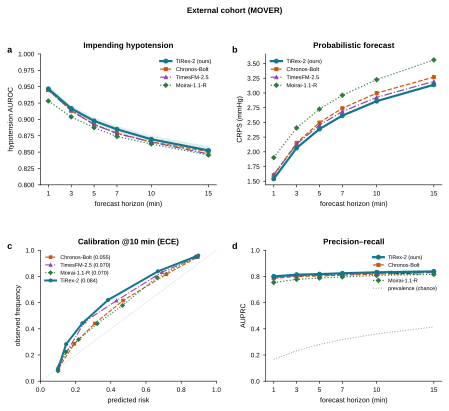
\includegraphics[width=\textwidth]{FigS_zeroshot_mover.png}
\caption{\textbf{External-cohort (MOVER) zero-shot foundation-model benchmark.}
TiRex-2 versus Chronos-Bolt, TimesFM-2.5 and Moirai-1.1-R on hypotension
AUROC, CRPS, calibration and AUPRC across horizons on the independent MOVER
cohort. The development-cohort ranking (Fig.~\ref{fig:zeroshot}) is
reproduced. Values in Table~\ref{tab:zeroshot_mover}.}
\label{fig:zeroshot_mover}
\end{figure}

% ---------- Supplementary Fig S2 : per-fold training curves ----------
\begin{figure}[H]
\centering
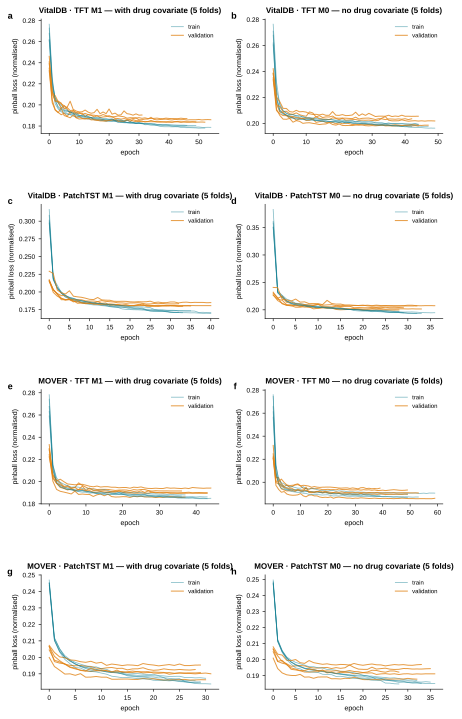
\includegraphics[width=\textwidth]{FigS_training_curves.png}
\caption{\textbf{Per-fold training and validation curves for the task-trained
baselines.} TFT and PatchTST across the 5 subject-level folds on both
cohorts, confirming convergence without overfitting.}
\label{fig:training_curves}
\end{figure}

% ---------- Table 2 : Classification vs supervised comparators ----------
\begin{table}[t]
\centering\footnotesize
\caption{\textbf{Impending-hypotension classification by zero-shot TiRex-2 on VitalDB, with external literature comparators.} M1 = with known-future drug covariate; M0 = without. Operating characteristics at fixed specificity $\geq$0.90. Kapral and Zhu columns are published external-VitalDB AUROC values (literature references, not re-executed). AUROC here is computed on the full development cohort by subject-level 5-fold out-of-fold cross-validation (all 2{,}665 subjects); the head-to-head comparisons in the main-text tables use matched evaluation windows common to all models on the held-out split, which shifts individual AUROC values by up to $\approx$0.005 (e.g.\ 7-min 0.908 here vs 0.905 matched). Values are not pooled across aggregations.}
\label{tab:classification}
\resizebox{\textwidth}{!}{%
\begin{tabular}{lccccccc}
\toprule
Horizon (min) & AUROC M1 [95\% CI] & AUROC M0 & AUPRC M1 & ECE & Sens/PPV/NPV/F1 @sp$\geq$.9 & Kapral ext.\ AUROC \citep{Kapral2024} & Zhu ext.\ AUROC \citep{Zhu2026} \\
\midrule
1  & 0.985 [0.983, 0.987] & 0.986 & 0.736 & 0.122 & 0.99/0.41/1.00/0.58 & 0.960 & --- \\
3  & 0.955 [0.950, 0.959] & 0.953 & 0.737 & 0.103 & 0.92/0.46/0.99/0.61 & 0.945 & --- \\
5  & 0.930 [0.924, 0.935] & 0.925 & 0.718 & 0.089 & 0.84/0.51/0.98/0.63 & 0.903 & 0.897 \\
7  & 0.908 [0.902, 0.914] & 0.902 & 0.701 & 0.077 & 0.78/0.53/0.97/0.63 & 0.867 & --- \\
10 & 0.881 [0.875, 0.888] & 0.877 & 0.682 & 0.060 & 0.71/0.56/0.95/0.63 & --- & 0.862 \\
15 & 0.854 [0.846, 0.862] & 0.852 & 0.672 & 0.041 & 0.64/0.60/0.92/0.62 & --- & 0.822 \\
\bottomrule
\end{tabular}}
\end{table}

% ---------- Table 3 : Operating characteristics ----------
\begin{table}[t]
\centering\footnotesize
\caption{\textbf{Early-warning operating characteristics of zero-shot TiRex-2 on VitalDB} at a fixed high-specificity operating point ($\geq$0.90). Calibration reported as expected calibration error (ECE).}
\label{tab:opchar}
\begin{tabular}{lccccc}
\toprule
Horizon (min) & Sensitivity & PPV & NPV & F1 & ECE \\
\midrule
1  & 0.99 & 0.41 & 1.00 & 0.58 & 0.122 \\
3  & 0.92 & 0.46 & 0.99 & 0.61 & 0.103 \\
5  & 0.84 & 0.51 & 0.98 & 0.63 & 0.089 \\
7  & 0.78 & 0.53 & 0.97 & 0.63 & 0.077 \\
10 & 0.71 & 0.56 & 0.95 & 0.63 & 0.060 \\
15 & 0.64 & 0.60 & 0.92 & 0.62 & 0.041 \\
\bottomrule
\end{tabular}
\end{table}

% ---------- Table 5 : Matched probabilistic forecasting accuracy ----------
\begin{table}[t]
\centering\footnotesize
\caption{\textbf{Matched probabilistic-forecasting accuracy on identical VitalDB windows} (M1, with drug covariate). CRPS and MAE for zero-shot TiRex-2 versus task-trained TFT and PatchTST (5-fold out-of-fold). Bold marks the best (lowest) value at each horizon.}
\label{tab:forecast}
\begin{tabular}{lcccccc}
\toprule
& \multicolumn{3}{c}{CRPS} & \multicolumn{3}{c}{MAE (mmHg)} \\
\cmidrule(lr){2-4}\cmidrule(lr){5-7}
Horizon (min) & TiRex-2 & TFT & PatchTST & TiRex-2 & TFT & PatchTST \\
\midrule
1  & \textbf{1.251} & 1.311 & 1.281 & \textbf{3.03} & 3.15 & 3.10 \\
3  & 1.827 & 1.779 & \textbf{1.726} & 4.46 & 4.35 & \textbf{4.24} \\
5  & 2.221 & 2.071 & \textbf{2.004} & 5.46 & 5.11 & \textbf{4.97} \\
7  & 2.515 & 2.273 & \textbf{2.200} & 6.20 & 5.65 & \textbf{5.48} \\
10 & 2.839 & 2.482 & \textbf{2.407} & 7.01 & 6.20 & \textbf{6.02} \\
15 & 3.213 & 2.716 & \textbf{2.656} & 7.95 & 6.82 & \textbf{6.68} \\
\bottomrule
\end{tabular}
\end{table}

% ---------- Table 7 : Cross-dataset transfer ----------
\begin{table}[t]
\centering\footnotesize
\caption{\textbf{Cross-dataset transfer (hypotension AUROC), covariate-free, both cohorts harmonised to 60 s cadence.} In-domain = held-out 5-fold out-of-fold; ``trained MOVER''/``trained VitalDB'' = all-train checkpoint applied across cohorts. Bold marks the best model on each test cohort at each horizon. On case-clustered bootstrap paired tests against zero-shot TiRex-2 (2{,}000 resamples), TiRex-2's advantage over the VitalDB-transferred baselines on MOVER was significant at 1 and 15~min ($+0.007$, $p<0.001$ vs transferred TFT at both), while its differences from the in-domain-trained models were small and mostly within the 95\% CI (all $|\Delta\text{AUROC}|\leq0.012$).}
\label{tab:transfer}
\resizebox{\textwidth}{!}{%
\begin{tabular}{llcccccc}
\toprule
Test cohort & Model (training source) & 1 min & 3 min & 5 min & 7 min & 10 min & 15 min \\
\midrule
\multirow{5}{*}{VitalDB}
 & TiRex-2 (zero-shot)      & \textbf{0.986} & \textbf{0.953} & \textbf{0.924} & \textbf{0.900} & \textbf{0.872} & \textbf{0.846} \\
 & TFT (in-domain)          & 0.983 & 0.945 & 0.913 & 0.888 & 0.858 & 0.831 \\
 & TFT (trained MOVER)      & 0.964 & 0.924 & 0.897 & 0.874 & 0.849 & 0.825 \\
 & PatchTST (in-domain)     & 0.982 & 0.947 & 0.920 & 0.897 & 0.870 & \textbf{0.846} \\
 & PatchTST (trained MOVER) & 0.967 & 0.928 & 0.900 & 0.877 & 0.851 & 0.832 \\
\midrule
\multirow{5}{*}{MOVER}
 & TiRex-2 (zero-shot)       & \textbf{0.948} & 0.919 & 0.899 & 0.886 & 0.872 & 0.855 \\
 & TFT (in-domain)           & 0.945 & \textbf{0.922} & \textbf{0.903} & \textbf{0.889} & 0.876 & 0.860 \\
 & TFT (trained VitalDB)     & 0.940 & 0.914 & 0.895 & 0.881 & 0.866 & 0.846 \\
 & PatchTST (in-domain)      & 0.945 & 0.919 & 0.901 & 0.888 & \textbf{0.877} & \textbf{0.862} \\
 & PatchTST (trained VitalDB)& 0.939 & 0.912 & 0.895 & 0.881 & 0.868 & 0.851 \\
\bottomrule
\end{tabular}}
\end{table}

% ---------- Supplementary Table S1 : Zero-shot FM AUROC on MOVER ----------
\begin{table}[t]
\centering\footnotesize
\caption{\textbf{Matched hypotension AUROC among zero-shot time-series foundation models on the external MOVER cohort} ($n=1{,}827$ subjects). All evaluated zero-shot; only TiRex-2 ingests the known-future drug-infusion covariate. Bold marks the best model at each horizon; the development-cohort ranking (Table~\ref{tab:zeroshot}) is reproduced.}
\label{tab:zeroshot_mover}
\begin{tabular}{lcccc}
\toprule
Horizon (min) & TiRex-2 [95\% CI] & Chronos-Bolt [95\% CI] & TimesFM-2.5 [95\% CI] & Moirai-1.1-R [95\% CI] \\
\midrule
1  & \textbf{0.947} [0.943, 0.951] & 0.945 [0.941, 0.949] & 0.945 [0.941, 0.949] & 0.928 [0.924, 0.933] \\
3  & \textbf{0.917} [0.912, 0.921] & 0.913 [0.909, 0.918] & 0.914 [0.909, 0.919] & 0.904 [0.899, 0.910] \\
5  & \textbf{0.898} [0.893, 0.903] & 0.892 [0.887, 0.897] & 0.892 [0.887, 0.897] & 0.887 [0.882, 0.893] \\
7  & \textbf{0.885} [0.880, 0.890] & 0.879 [0.874, 0.885] & 0.878 [0.873, 0.884] & 0.874 [0.868, 0.880] \\
10 & \textbf{0.870} [0.864, 0.875] & 0.866 [0.860, 0.871] & 0.865 [0.860, 0.871] & 0.863 [0.857, 0.869] \\
15 & \textbf{0.853} [0.847, 0.859] & 0.851 [0.845, 0.857] & 0.847 [0.841, 0.854] & 0.846 [0.839, 0.852] \\
\bottomrule
\end{tabular}
\end{table}

% ---------- Table S2 : Paired significance tests ----------
\begin{table}[t]
\centering\footnotesize
\caption{\textbf{Paired significance tests} (case-clustered bootstrap, 2{,}000 resamples). Covariate benefit is the CRPS reduction in transition windows at 7 min; AUROC differences are paired on identical windows. Foundation-model rows are quoted to three decimals; Supplementary Table~\ref{tab:fm_pairwise} gives the same quantities to four decimals from an independent bootstrap summary, so a few point estimates differ by $\leq$0.001 from the rounded values here. $^{***}p<0.001$, $^{**}p<0.01$, n.s.\ not significant.}
\label{tab:stats}
\begin{tabular}{p{3cm}lccc}
\toprule
Test & Comparison & Estimate & 95\% CI & $p$ \\
\midrule
\multirow{3}{2.9cm}{\raggedright Covariate benefit vs 0 (CE, 7 min)}
 & TiRex-2   & $+1.15\%$  & [$+0.84$, $+1.47$]   & $<$0.001$^{***}$ \\
 & TFT       & $+7.12\%$  & [$+6.57$, $+7.68$]   & $<$0.001$^{***}$ \\
 & PatchTST  & $+12.48\%$ & [$+11.87$, $+13.10$] & $<$0.001$^{***}$ \\
\midrule
\multirow{3}{2.9cm}{\raggedright Covariate benefit, between-model (7 min)}
 & TFT $-$ TiRex-2      & $+5.98\%$  & [$+5.38$, $+6.54$]   & $<$0.001$^{***}$ \\
 & PatchTST $-$ TiRex-2 & $+11.33\%$ & [$+10.70$, $+11.97$] & $<$0.001$^{***}$ \\
 & PatchTST $-$ TFT     & $+5.35\%$  & [$+4.83$, $+5.86$]   & $<$0.001$^{***}$ \\
\midrule
\multirow{9}{2.9cm}{\raggedright Zero-shot AUROC difference (Table~\ref{tab:zeroshot})}
 & TiRex-2 $-$ Chronos-Bolt @5min  & $+0.008$ & [$+0.005$, $+0.011$] & $<$0.001$^{***}$ \\
 & TiRex-2 $-$ Chronos-Bolt @10min & $+0.009$ & [$+0.006$, $+0.012$] & $<$0.001$^{***}$ \\
 & TiRex-2 $-$ Chronos-Bolt @15min & $+0.009$ & [$+0.005$, $+0.012$] & $<$0.001$^{***}$ \\
 & TiRex-2 $-$ TimesFM-2.5 @5min   & $+0.008$ & [$+0.006$, $+0.011$] & $<$0.001$^{***}$ \\
 & TiRex-2 $-$ TimesFM-2.5 @10min  & $+0.008$ & [$+0.004$, $+0.011$] & $<$0.001$^{***}$ \\
 & TiRex-2 $-$ TimesFM-2.5 @15min  & $+0.005$ & [$+0.002$, $+0.009$] & $<$0.001$^{***}$ \\
 & TiRex-2 $-$ Moirai-1.1-R @5min  & $+0.007$ & [$+0.003$, $+0.010$] & $<$0.001$^{***}$ \\
 & TiRex-2 $-$ Moirai-1.1-R @10min & $+0.010$ & [$+0.007$, $+0.014$] & $<$0.001$^{***}$ \\
 & TiRex-2 $-$ Moirai-1.1-R @15min & $+0.012$ & [$+0.008$, $+0.016$] & $<$0.001$^{***}$ \\
\midrule
\multirow{6}{2.9cm}{\raggedright Trained-SOTA AUROC difference (Table~\ref{tab:matched})}
 & TiRex-2 $-$ TFT @5min       & $+0.006$ & [$+0.002$, $+0.009$] & 0.002$^{**}$ \\
 & TiRex-2 $-$ TFT @7min       & $+0.002$ & [$-0.002$, $+0.005$] & 0.337 n.s. \\
 & TiRex-2 $-$ TFT @15min      & $-0.011$ & [$-0.016$, $-0.007$] & $<$0.001$^{***}$ \\
 & TiRex-2 $-$ PatchTST @5min  & $-0.008$ & [$-0.012$, $-0.005$] & $<$0.001$^{***}$ \\
 & TiRex-2 $-$ PatchTST @7min  & $-0.013$ & [$-0.017$, $-0.010$] & $<$0.001$^{***}$ \\
 & TiRex-2 $-$ PatchTST @15min & $-0.026$ & [$-0.031$, $-0.022$] & $<$0.001$^{***}$ \\
\bottomrule
\end{tabular}
\end{table}


% ---------- Supplementary Table : FM pairwise significance ----------
\begin{table}[ht]
\centering\footnotesize
\caption{\textbf{Paired hypotension-AUROC differences among zero-shot foundation models on VitalDB, all horizons.} TiRex-2 minus each univariate comparator, on identical windows; case-clustered bootstrap (2{,}000 resamples) 95\% CI and two-sided $p$. Positive favours TiRex-2. Extends the main comparison, which quoted only 5/10/15~min, to all six horizons; note the 1-min tie with TimesFM-2.5.}
\label{tab:fm_pairwise}
\begin{tabular}{llrrr}
\toprule
Horizon (min) & Comparison & $\Delta$AUROC & 95\% CI & $p$ \\
\midrule
1 & TiRex-2 $-$ Chronos-Bolt & +0.0011 & [+0.0003, +0.0026] & 0.009 \\
1 & TiRex-2 $-$ TimesFM-2.5 & -0.0004 & [-0.0013, +0.0008] & 0.640 \\
1 & TiRex-2 $-$ Moirai-1.1-R & +0.0087 & [+0.0063, +0.0123] & $<$0.001 \\
3 & TiRex-2 $-$ Chronos-Bolt & +0.0058 & [+0.0029, +0.0081] & $<$0.001 \\
3 & TiRex-2 $-$ TimesFM-2.5 & +0.0052 & [+0.0025, +0.0076] & $<$0.001 \\
3 & TiRex-2 $-$ Moirai-1.1-R & +0.0093 & [+0.0049, +0.0117] & $<$0.001 \\
5 & TiRex-2 $-$ Chronos-Bolt & +0.0072 & [+0.0047, +0.0109] & $<$0.001 \\
5 & TiRex-2 $-$ TimesFM-2.5 & +0.0083 & [+0.0056, +0.0114] & $<$0.001 \\
5 & TiRex-2 $-$ Moirai-1.1-R & +0.0070 & [+0.0033, +0.0100] & $<$0.001 \\
7 & TiRex-2 $-$ Chronos-Bolt & +0.0079 & [+0.0049, +0.0113] & $<$0.001 \\
7 & TiRex-2 $-$ TimesFM-2.5 & +0.0077 & [+0.0049, +0.0112] & $<$0.001 \\
7 & TiRex-2 $-$ Moirai-1.1-R & +0.0090 & [+0.0047, +0.0121] & $<$0.001 \\
10 & TiRex-2 $-$ Chronos-Bolt & +0.0096 & [+0.0056, +0.0126] & $<$0.001 \\
10 & TiRex-2 $-$ TimesFM-2.5 & +0.0083 & [+0.0042, +0.0110] & $<$0.001 \\
10 & TiRex-2 $-$ Moirai-1.1-R & +0.0109 & [+0.0062, +0.0144] & $<$0.001 \\
15 & TiRex-2 $-$ Chronos-Bolt & +0.0094 & [+0.0050, +0.0125] & $<$0.001 \\
15 & TiRex-2 $-$ TimesFM-2.5 & +0.0064 & [+0.0020, +0.0090] & $<$0.001 \\
15 & TiRex-2 $-$ Moirai-1.1-R & +0.0122 & [+0.0079, +0.0166] & $<$0.001 \\
\bottomrule
\end{tabular}
\end{table}

% ---------- Supplementary Table : MOVER operating characteristics ----------
\begin{table}[ht]
\centering\footnotesize
\caption{\textbf{Zero-shot TiRex-2 operating characteristics on the external MOVER cohort.} Discrimination (AUROC, AUPRC with case-clustered bootstrap 95\% CI) and operating-point metrics at a fixed specificity $\geq$0.90, by horizon. Under MOVER's 2--3$\times$ higher hypotension prevalence, positive predictive value (PPV) rises substantially relative to the lower-prevalence development cohort. As with the VitalDB tables, MOVER AUROC values differ by up to $\approx$0.005 across tables (e.g.\ 1-min 0.946 here vs 0.947 in Table~\ref{tab:external}) because each table applies a different aggregation (full-cohort out-of-fold, matched windows, or the 20\% test split); values are reported per aggregation and not pooled.}
\label{tab:mover_opchar}
\begin{tabular}{lrrrrrrr}
\toprule
Horizon (min) & Prevalence & AUROC (95\% CI) & AUPRC (95\% CI) & Sens. & PPV & NPV & F1 \\
\midrule
1 & 0.167 & 0.946 [0.943, 0.951] & 0.799 [0.782, 0.813] & 0.909 & 0.646 & 0.980 & 0.755 \\
3 & 0.233 & 0.915 [0.912, 0.921] & 0.809 [0.796, 0.822] & 0.813 & 0.711 & 0.941 & 0.759 \\
5 & 0.281 & 0.897 [0.893, 0.903] & 0.814 [0.802, 0.826] & 0.755 & 0.747 & 0.904 & 0.751 \\
7 & 0.317 & 0.884 [0.879, 0.890] & 0.820 [0.810, 0.832] & 0.721 & 0.770 & 0.874 & 0.745 \\
10 & 0.361 & 0.868 [0.864, 0.875] & 0.828 [0.818, 0.839] & 0.687 & 0.795 & 0.836 & 0.737 \\
15 & 0.414 & 0.850 [0.846, 0.859] & 0.834 [0.825, 0.845] & 0.649 & 0.821 & 0.784 & 0.725 \\
\bottomrule
\end{tabular}
\end{table}

% ---------- Supplementary Table : covariate benefit by stratum ----------
\begin{table}[ht]
\centering\footnotesize
\caption{\textbf{TiRex-2 covariate benefit by window stratum on VitalDB (CRPS reduction, M0$\rightarrow$M1).} Percent CRPS reduction from adding the known-future drug covariate, with case-clustered bootstrap 95\% CI, split into transition windows (drug effect-site concentration changes over the horizon) and steady windows (it does not). The benefit is positive and significant only in transition windows and is absent or slightly negative in steady windows, consistent with the model exploiting genuinely informative changes in the planned infusion rather than reacting to the outcome.}
\label{tab:covariate_split}
\begin{tabular}{lrrr}
\toprule
Horizon (min) & Transition \% [95\% CI] & Steady \% [95\% CI] & All \% \\
\midrule
1 & -0.34 [-0.82, +0.08] & -0.58 [-0.94, -0.25] & -0.36 \\
3 & +0.41 [+0.05, +0.72] & -0.53 [-0.81, -0.25] & +0.15 \\
5 & +0.87 [+0.55, +1.18] & -0.47 [-0.74, -0.19] & +0.47 \\
7 & +1.15 [+0.83, +1.46] & -0.50 [-0.80, -0.23] & +0.66 \\
10 & +1.42 [+1.11, +1.73] & -0.56 [-0.86, -0.28] & +0.86 \\
15 & +1.17 [+0.86, +1.48] & -0.67 [-0.97, -0.38] & +0.65 \\
\bottomrule
\end{tabular}
\end{table}

% ---------- Supplementary Table : naive baselines (autocorrelation floor) ----------
\begin{table}[ht]
\centering\footnotesize
\caption{\textbf{Naive persistence baseline versus zero-shot TiRex-2, both cohorts, identical test windows.} Persistence ranks impending hypotension by the last observed MAP (a monotone transform, so its AUROC equals that of a ``last MAP\,$<$\,65'' alarm); scored on a held-out 20\% subject-level test split with case-clustered bootstrap 95\% CI. TiRex-2 is scored on the same split. $\Delta$ = TiRex-2 $-$ persistence. Because MAP is strongly autocorrelated over short intervals, the persistence floor is high at the shortest horizons---on MOVER's 60 s cadence it reaches AUROC 0.997 at 1 min---and the skill of the learned models above it widens with horizon. A MAP-trend logistic (last MAP + recent slope) gave AUROC within 0.001 of persistence at every horizon and is omitted for brevity.}
\label{tab:naive}
\begin{tabular}{lrrrrr}
\toprule
Horizon (min) & Prevalence & Persistence AUROC (95\% CI) & Persist.\ AUPRC & TiRex-2 AUROC & $\Delta$ \\
\midrule
\multicolumn{6}{l}{\textit{VitalDB (development, 15 s cadence)}}\\
1 & 0.054 & 0.987 [0.985, 0.989] & 0.738 & 0.985 & -0.003 \\
3 & 0.084 & 0.951 [0.946, 0.955] & 0.710 & 0.957 & +0.006 \\
5 & 0.106 & 0.921 [0.915, 0.926] & 0.684 & 0.929 & +0.009 \\
7 & 0.124 & 0.893 [0.887, 0.900] & 0.663 & 0.904 & +0.011 \\
10 & 0.150 & 0.860 [0.853, 0.868] & 0.642 & 0.876 & +0.016 \\
15 & 0.184 & 0.827 [0.819, 0.836] & 0.629 & 0.847 & +0.020 \\
\midrule
\multicolumn{6}{l}{\textit{MOVER (external, 60 s cadence)}}\\
1 & 0.167 & 0.997 [0.997, 0.998] & 0.957 & 0.948 & -0.049 \\
3 & 0.233 & 0.952 [0.948, 0.957] & 0.902 & 0.917 & -0.036 \\
5 & 0.281 & 0.918 [0.913, 0.924] & 0.872 & 0.898 & -0.021 \\
7 & 0.318 & 0.892 [0.886, 0.898] & 0.854 & 0.885 & -0.007 \\
10 & 0.361 & 0.866 [0.860, 0.873] & 0.844 & 0.869 & +0.003 \\
15 & 0.414 & 0.841 [0.834, 0.848] & 0.839 & 0.851 & +0.010 \\
\bottomrule
\end{tabular}
\end{table}

% ---------- Supplementary Table : persistence vs all learned models ----------
\begin{table}[ht]
\centering\footnotesize
\caption{\textbf{Naive persistence floor versus all learned models (hypotension AUROC), identical test windows, both cohorts.} Persistence ranks by last observed MAP; all models---persistence, TiRex-2, TFT and PatchTST---scored on the same held-out 20\% subject-level test split (not the full-cohort out-of-fold set), so AUROC values here differ slightly (typically within $\approx$0.005, mostly lower for the trained models) from the full-cohort figures in Table~\ref{tab:matched}; the point of this table is the within-split ordering against persistence, not absolute values. Bold marks the best model at each horizon (persistence is not overtaken through 5~min on MOVER; the 7~min MOVER row is a three-way tie at 0.892 with TiRex-2 just below). On VitalDB (15 s cadence) persistence is best only at 1 min; on MOVER (60 s cadence) it is best through 5 min and the learned models---foundation and task-trained alike---overtake it only from 10 min. The distinctive value of any learned model on the external cohort is therefore concentrated at the longer horizons.}
\label{tab:naive_learned}
\begin{tabular}{lrrrr}
\toprule
Horizon (min) & Persistence & TiRex-2 & TFT & PatchTST \\
\midrule
\multicolumn{5}{l}{\textit{VitalDB (development, 15 s cadence; TFT/PatchTST 5-fold OOF)}}\\
1 & \textbf{0.987} & 0.985 & 0.981 & 0.982 \\
3 & 0.951 & \textbf{0.957} & 0.946 & 0.954 \\
5 & 0.921 & 0.929 & 0.921 & \textbf{0.936} \\
7 & 0.893 & 0.904 & 0.898 & \textbf{0.914} \\
10 & 0.860 & 0.876 & 0.876 & \textbf{0.895} \\
15 & 0.827 & 0.847 & 0.856 & \textbf{0.872} \\
\midrule
\multicolumn{5}{l}{\textit{MOVER (external, 60 s cadence; TFT/PatchTST in-domain 5-fold OOF)}}\\
1 & \textbf{0.997} & 0.948 & 0.943 & 0.948 \\
3 & \textbf{0.952} & 0.917 & 0.920 & 0.920 \\
5 & \textbf{0.918} & 0.898 & 0.904 & 0.905 \\
7 & \textbf{0.892} & 0.885 & 0.892 & 0.892 \\
10 & 0.866 & 0.869 & 0.878 & \textbf{0.879} \\
15 & 0.841 & 0.851 & \textbf{0.865} & 0.864 \\
\bottomrule
\end{tabular}
\end{table}

% ---------- Supplementary Table : calibration and recalibration ----------
\begin{table}[ht]
\centering\footnotesize
\caption{\textbf{Calibration of zero-shot TiRex-2 (M1) and its correction by post-hoc recalibration, both cohorts.} Expected calibration error (ECE, 10 equal-count bins) on the held-out test split, before and after isotonic recalibration fitted on the disjoint development split; calibration slope and intercept from a logistic recalibration model (slope 1 = ideal; $>$1 indicates under-dispersion, i.e.\ predictions not extreme enough). The zero-shot risk scores are mildly under-dispersed (slopes 1.1--1.7), consistent with the coarse nine-level quantile grid compressing risk toward the middle, and a single monotone recalibration step---label-free at inference, requiring only a one-off fit on a labelled subset---reduces ECE to $\leq$0.012 at every horizon on both cohorts. The largest raw ECE (0.122 at VitalDB 1 min; 0.123 at MOVER 15 min) is fully correctable.}
\label{tab:calibration}
\begin{tabular}{lrrrr}
\toprule
Horizon (min) & ECE (raw) & ECE (recalibrated) & Calib.\ slope & Calib.\ intercept \\
\midrule
\multicolumn{5}{l}{\textit{VitalDB (development, 15 s cadence)}}\\
1 & 0.122 & 0.001 & 1.74 & -2.77 \\
3 & 0.103 & 0.001 & 1.38 & -1.34 \\
5 & 0.090 & 0.003 & 1.30 & -0.91 \\
7 & 0.077 & 0.005 & 1.24 & -0.65 \\
10 & 0.059 & 0.007 & 1.18 & -0.42 \\
15 & 0.040 & 0.008 & 1.13 & -0.14 \\
\midrule
\multicolumn{5}{l}{\textit{MOVER (external, 60 s cadence)}}\\
1 & 0.078 & 0.007 & 1.37 & -0.72 \\
3 & 0.054 & 0.004 & 1.35 & +0.05 \\
5 & 0.062 & 0.011 & 1.34 & +0.43 \\
7 & 0.063 & 0.011 & 1.35 & +0.71 \\
10 & 0.085 & 0.011 & 1.35 & +1.00 \\
15 & 0.123 & 0.006 & 1.33 & +1.27 \\
\bottomrule
\end{tabular}
\end{table}

% ---------- Supplementary Figure : decision-curve analysis ----------
\begin{figure}[ht]
\centering
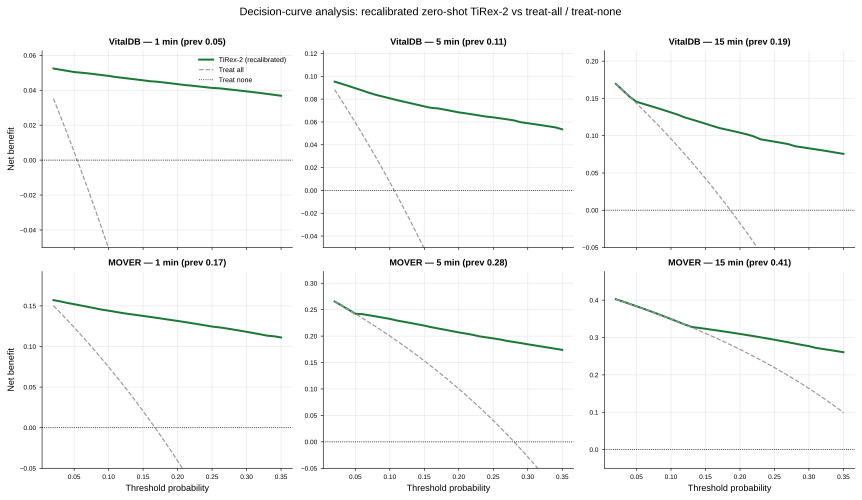
\includegraphics[width=\textwidth]{figs/FigS_decision_curves.png}
\caption{\textbf{Decision-curve analysis of recalibrated zero-shot TiRex-2, both cohorts.} Net benefit versus threshold probability at 1, 5 and 15~min on VitalDB (top) and MOVER (bottom), for the isotonic-recalibrated TiRex-2 risk against the two default strategies, treat-all (dashed) and treat-none (net benefit 0, dotted). The recalibrated model exceeded both references across essentially the whole clinically plausible threshold range on VitalDB (100\% of 2--35\% thresholds at 1 and 5~min; 91\% at 15~min) and over most of the range on MOVER (100\%/88\%/68\% at 1/5/15~min), the narrowing at MOVER 15~min reflecting the very high event prevalence (41\%), which raises the treat-all reference. Curves use the held-out test split with the isotonic map fitted on each cohort's disjoint development split.}
\label{fig:dca}
\end{figure}

% ==================== Explainability: what the zero-shot representations encode ====================
% ---------- Supplementary Figure : UMAP of per-window representations, VitalDB ----------
\begin{figure}[ht]
\centering
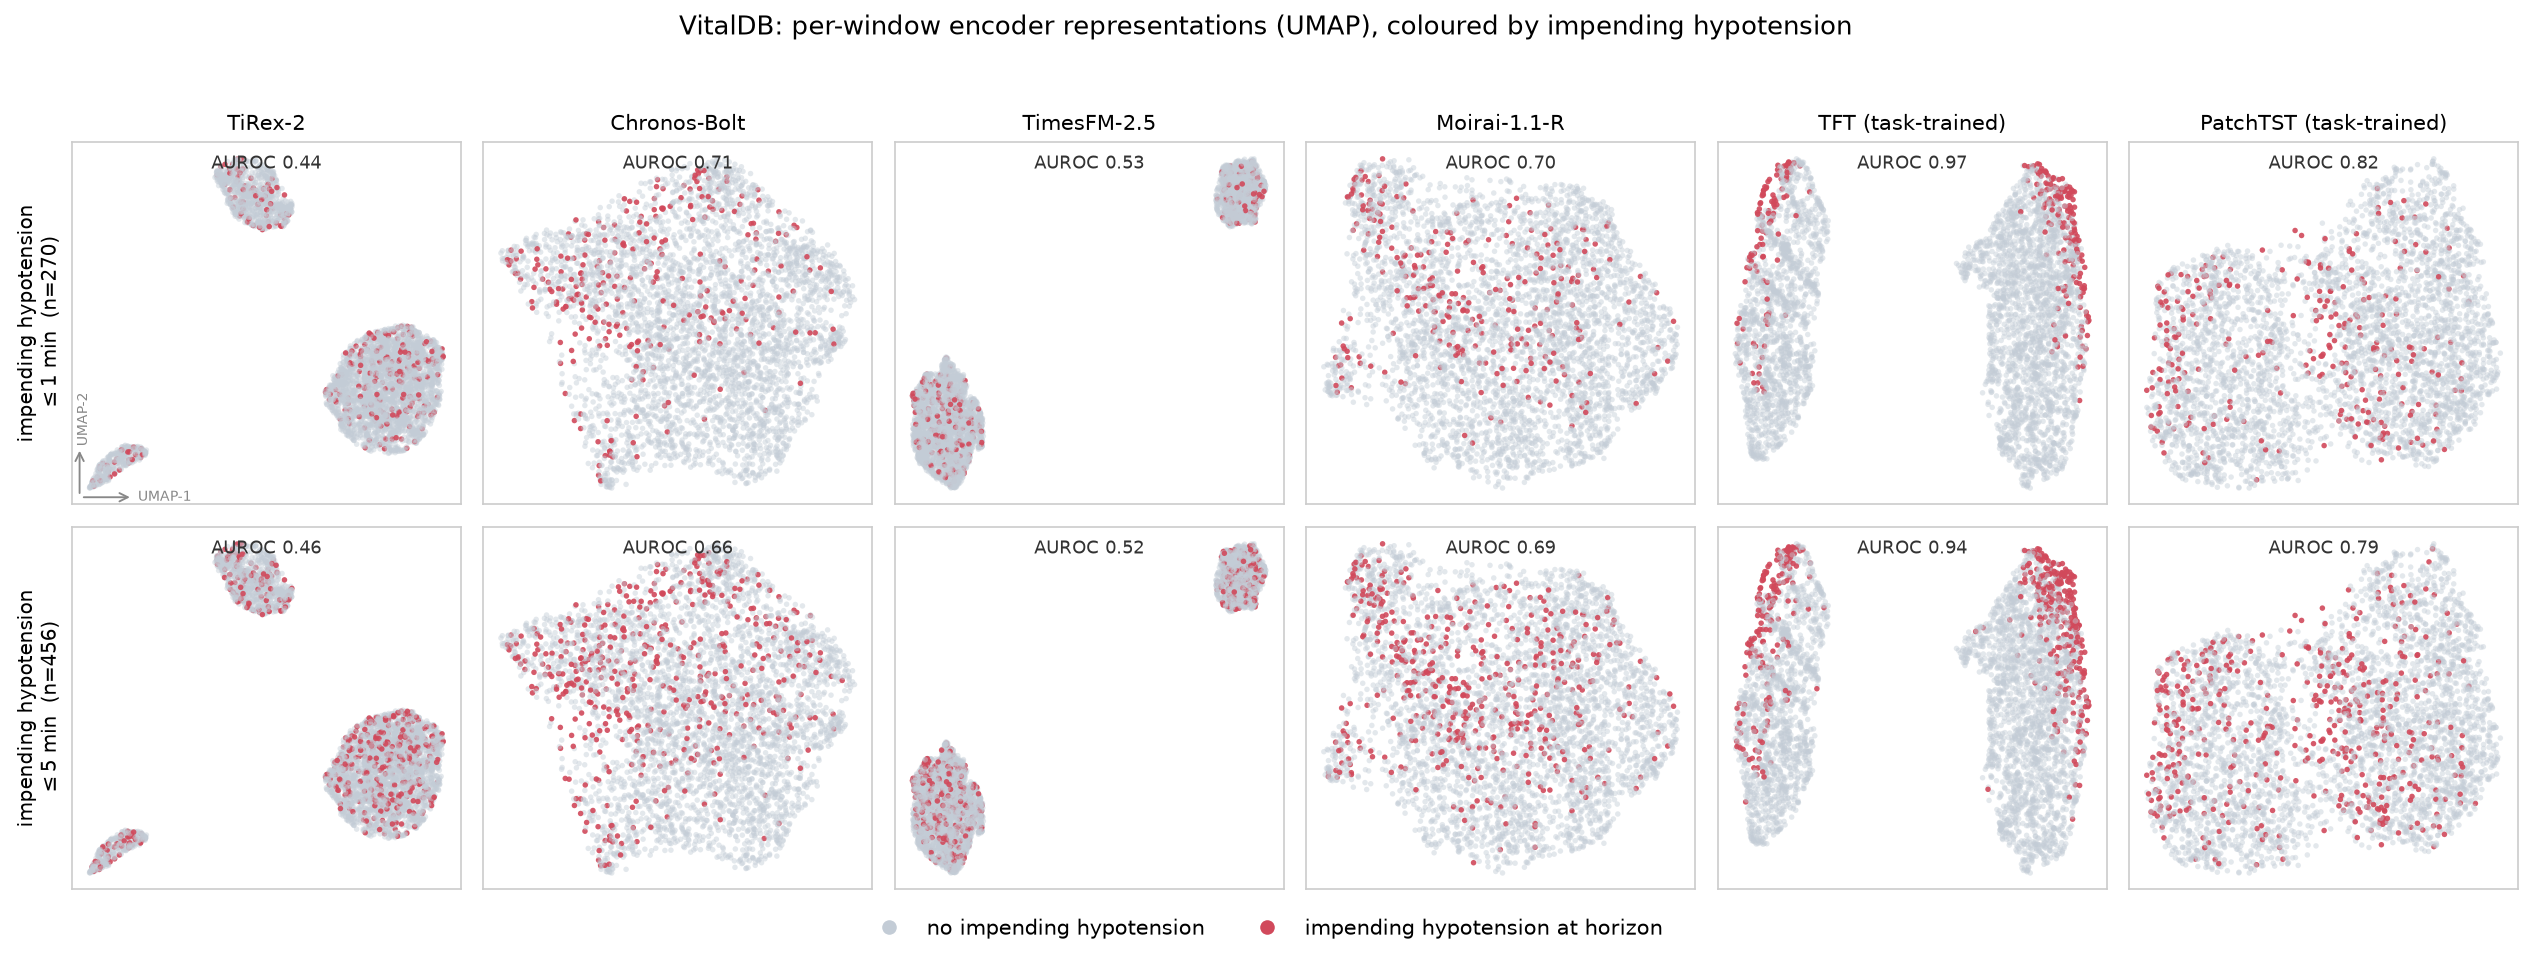
\includegraphics[width=\textwidth]{figs/FigS_umap_vitaldb.png}
\caption{\textbf{Per-window encoder representations on VitalDB, projected with UMAP and coloured by impending hypotension.} Each point is one forecast window; its position is a 2-D UMAP projection of that model's pooled penultimate-layer representation (standardised, Euclidean), and its colour marks whether MAP fell below 65~mmHg within the stated horizon (top row 1~min, bottom row 5~min; identical 4{,}000-window subsample across all models). The per-panel value is the AUROC of a subject-grouped linear probe for the same label (Supplementary Table~\ref{tab:probe_hypo}). Two distinct structures should not be conflated. (i)~The \emph{clinical} label appears as a diffuse colour \emph{gradient}, not as discrete clusters: red concentrates in a region of the manifold for the task-trained models (TFT, PatchTST) and, more weakly, for the univariate zero-shot models (Chronos, Moirai), but is spread at base rate for TiRex-2 and TimesFM-2.5. (ii)~The \emph{discrete} groupings visible in some panels (TiRex-2, TimesFM-2.5 split into separated islands) are \emph{not} clinical---they reflect embedding-activation magnitude or surgical context, not outcome (Supplementary Table~\ref{tab:cluster_char}). Notably the best forecaster, TiRex-2, shows the weakest colour gradient of all six models.}
\label{fig:umap_vitaldb}
\end{figure}

% ---------- Supplementary Figure : UMAP of per-window representations, MOVER ----------
\begin{figure}[ht]
\centering
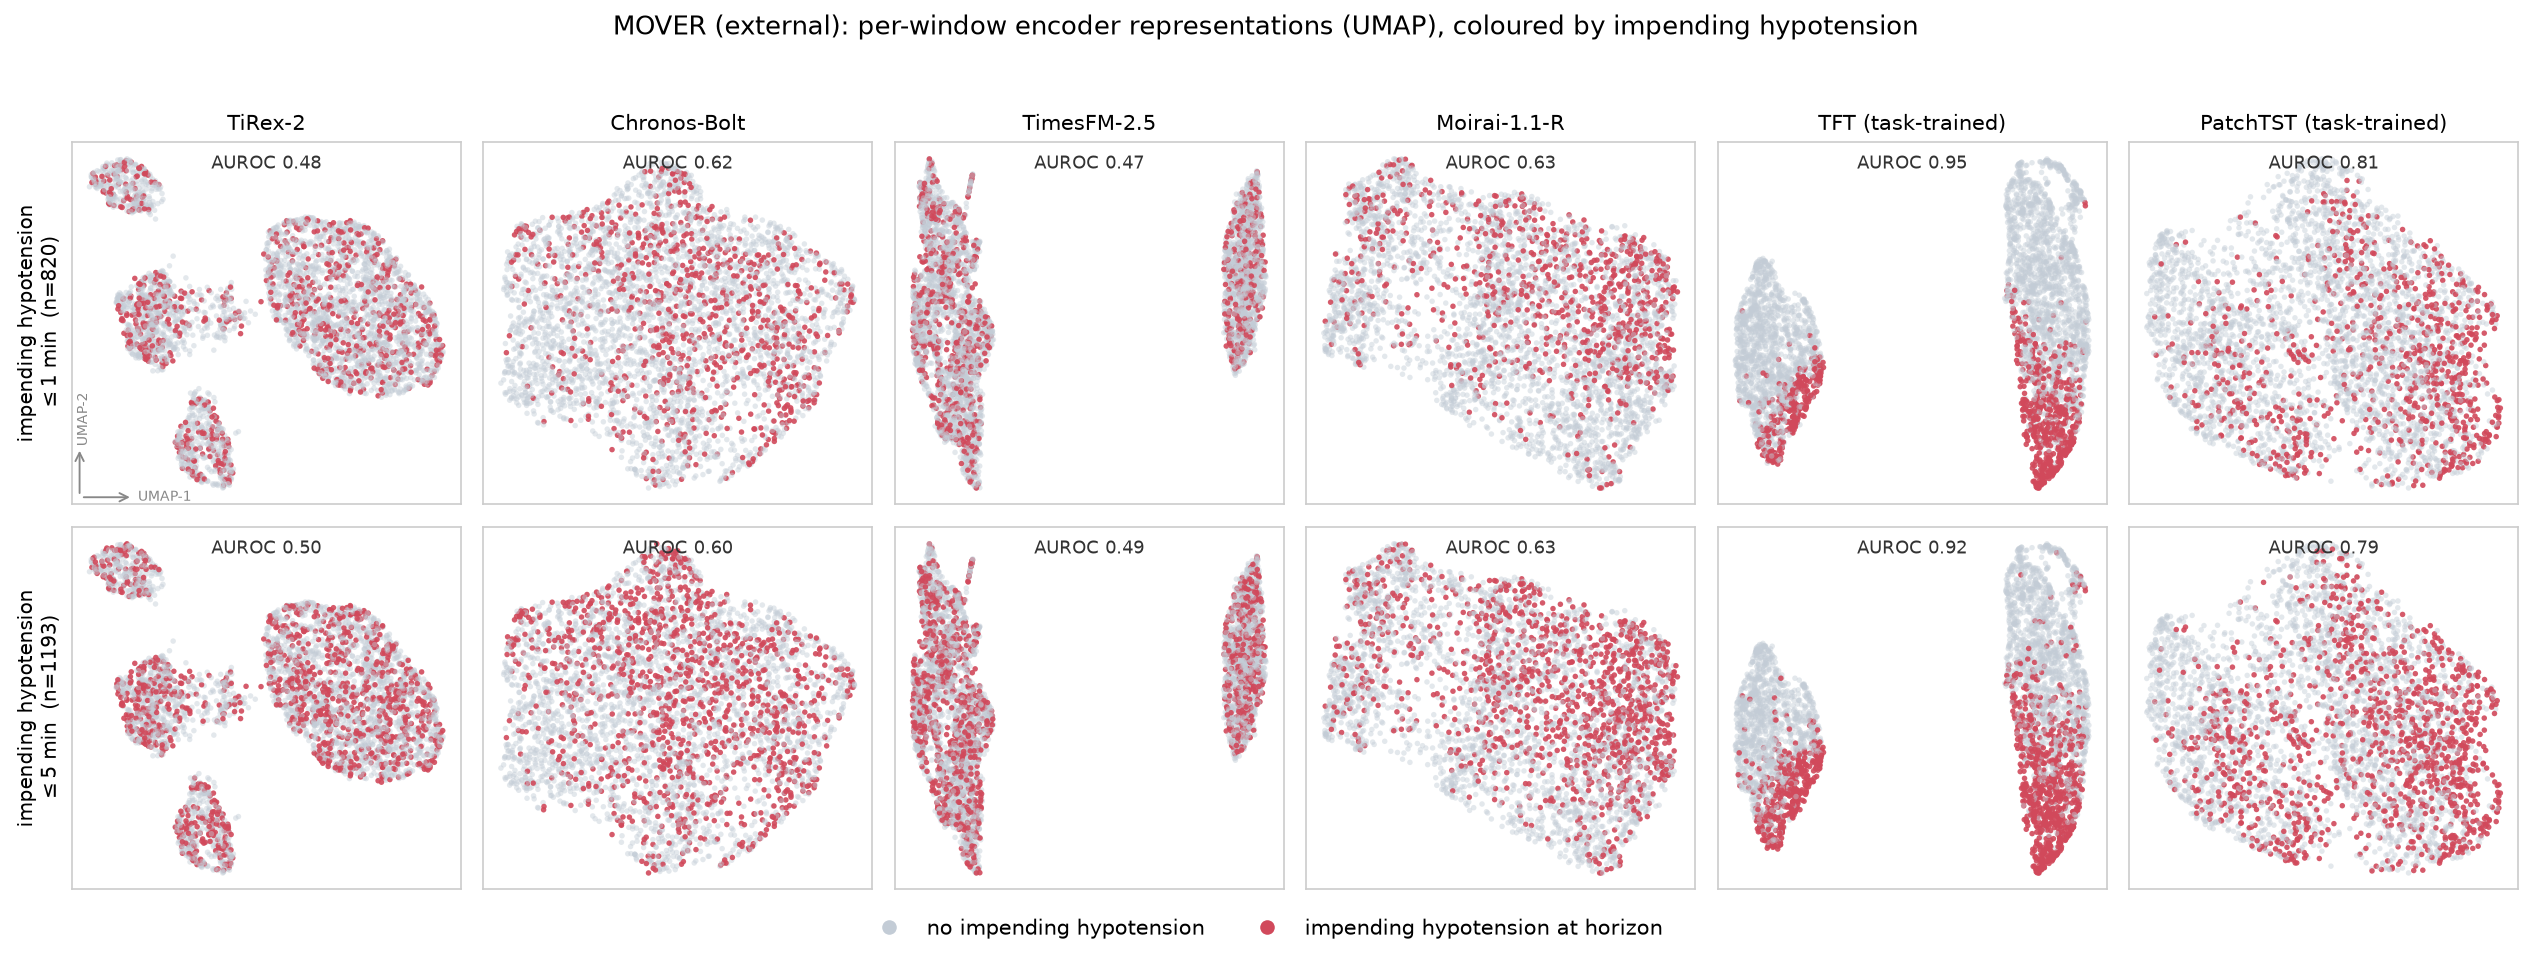
\includegraphics[width=\textwidth]{figs/FigS_umap_mover.png}
\caption{\textbf{Per-window encoder representations on the external MOVER cohort, projected with UMAP.} As Supplementary Fig.~\ref{fig:umap_vitaldb}, on the independent MOVER cohort (3{,}999-window subsample; 60~s cadence; higher hypotension prevalence). The pattern replicates externally: the model ordering by colour-gradient strength (probe AUROC) is unchanged---task-trained $>$ univariate zero-shot $>$ TiRex-2/TimesFM-2.5 at chance---and the non-clinical discrete islands persist for the same models.}
\label{fig:umap_mover}
\end{figure}

% ---------- Supplementary Figure : RSA / linear CKA ----------
\begin{figure}[ht]
\centering
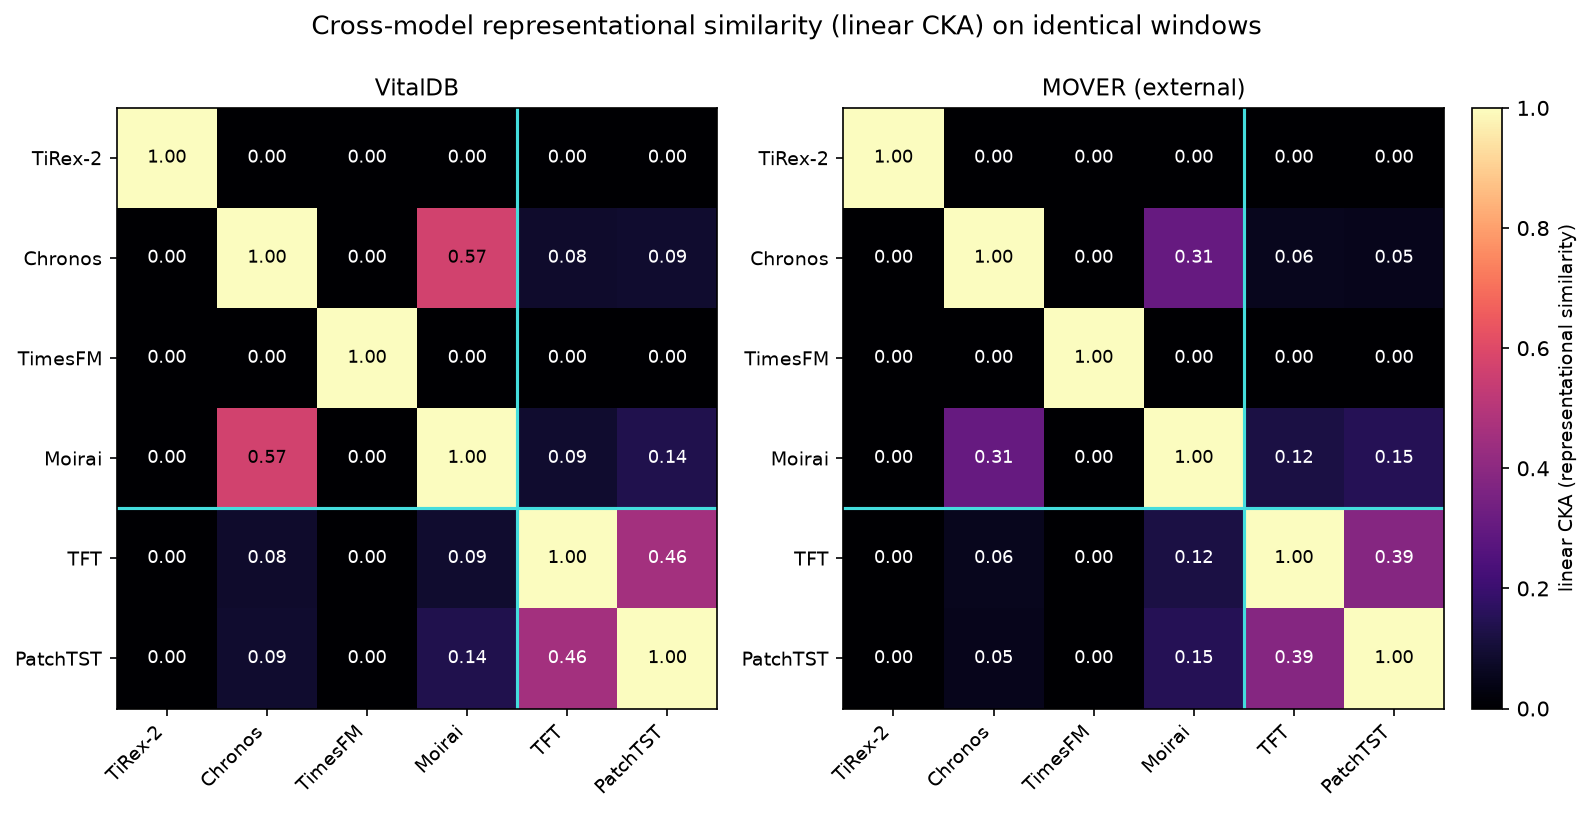
\includegraphics[width=\textwidth]{figs/FigS_rsa_cka.png}
\caption{\textbf{Cross-model representational similarity (linear CKA) on identical windows, both cohorts.} Linear centred kernel alignment between every pair of models' per-window representations, computed on the identical window subsample (dimension-agnostic, so it compares representations of different width). Cyan lines separate the zero-shot foundation models (upper-left block) from the task-trained baselines (lower-right). Cross-family similarity is near zero on both cohorts; the only substantial off-diagonal similarities are \emph{within} family---Chronos-Bolt$\leftrightarrow$Moirai (0.57 VitalDB) and TFT$\leftrightarrow$PatchTST (0.46)---while TiRex-2 and TimesFM-2.5 are nearly orthogonal to all other models. The four zero-shot models therefore do not share a common representational geometry, and none aligns with the task-trained models, even though several forecast comparably well.}
\label{fig:rsa_cka}
\end{figure}

% ---------- Supplementary Table : hypotension linear probe ----------
\begin{table}[ht]
\centering\footnotesize
\caption{\textbf{Linear separability of impending hypotension from per-window representations (subject-grouped probe).} AUROC (mean over 5 subject-grouped folds; per-fold s.d.\ $\leq$0.036 throughout) of an L2-regularised logistic probe predicting MAP$<$65~mmHg within each horizon from each model's frozen representation; no representation is fine-tuned. Area under the precision--recall curve is reported in the accompanying machine-readable table (\texttt{suppl\_probe\_hypotension.csv}). Windows are the identical subsample of Supplementary Figs.~\ref{fig:umap_vitaldb}--\ref{fig:umap_mover}, and folds are split by case so no subject appears in both train and test. Separability is a property of the \emph{representation}: it is highest for the task-trained models (which were optimised to expose exactly this label) and, among the zero-shot models, present but partial for the univariate Chronos-Bolt and Moirai and at chance for TiRex-2 and TimesFM-2.5. The ordering is stable across horizons and replicates on MOVER. Crucially it does not track forecasting skill---TiRex-2, the strongest forecaster, has the least task-separable representation.}
\label{tab:probe_hypo}
\begin{tabular}{llrrrrrr}
\toprule
& & \multicolumn{6}{c}{AUROC by horizon (min)} \\
\cmidrule(lr){3-8}
Cohort & Model & 1 & 2 & 3 & 5 & 10 & 15 \\
\midrule
\multicolumn{8}{l}{\textit{VitalDB (development)}}\\
& TiRex-2 & 0.441 & 0.455 & 0.462 & 0.464 & 0.479 & 0.485 \\
& Chronos-Bolt & 0.706 & 0.688 & 0.700 & 0.656 & 0.624 & 0.615 \\
& TimesFM-2.5 & 0.531 & 0.513 & 0.521 & 0.522 & 0.501 & 0.483 \\
& Moirai-1.1-R & 0.697 & 0.715 & 0.705 & 0.691 & 0.670 & 0.657 \\
& TFT (trained) & \textbf{0.974} & \textbf{0.964} & \textbf{0.954} & \textbf{0.939} & \textbf{0.911} & \textbf{0.892} \\
& PatchTST (trained) & 0.821 & 0.818 & 0.810 & 0.785 & 0.768 & 0.750 \\
\midrule
\multicolumn{8}{l}{\textit{MOVER (external)}}\\
& TiRex-2 & 0.485 & 0.486 & 0.503 & 0.504 & 0.481 & 0.482 \\
& Chronos-Bolt & 0.623 & 0.621 & 0.615 & 0.601 & 0.604 & 0.592 \\
& TimesFM-2.5 & 0.472 & 0.486 & 0.493 & 0.490 & 0.512 & 0.504 \\
& Moirai-1.1-R & 0.630 & 0.618 & 0.614 & 0.626 & 0.604 & 0.602 \\
& TFT (trained) & \textbf{0.951} & \textbf{0.938} & \textbf{0.925} & \textbf{0.915} & \textbf{0.896} & \textbf{0.884} \\
& PatchTST (trained) & 0.812 & 0.801 & 0.791 & 0.785 & 0.776 & 0.769 \\
\bottomrule
\end{tabular}
\end{table}

% ---------- Supplementary Table : continuous MAP trajectory probe ----------
\begin{table}[ht]
\centering\footnotesize
\caption{\textbf{Linear decodability of continuous hemodynamic state from per-window representations ($R^2$).} Cross-validated $R^2$ (subject-grouped ridge probe) predicting continuous mean arterial pressure quantities from each frozen representation: current MAP at the forecast origin, mean and minimum MAP over the next 5~min, mean MAP over the full horizon, and MAP slope over 5~min and the full horizon. Negative $R^2$ means the probe does worse than predicting the mean. This is the construct-valid test for a forecaster---whether its latent linearly encodes the hemodynamic trajectory---and the result is striking: only the task-trained TFT exposes MAP linearly ($R^2\!\approx\!0.8$--0.96 for current/near-future level), while the zero-shot foundation models are weak to negative, TiRex-2 included ($R^2\!\approx\!-0.08$, i.e.\ at chance). A forecaster's skill therefore resides in its full encoder$\rightarrow$decoder mapping conditioned on covariates, not in a linearly-decodable summary of its pooled penultimate state, which discards the temporal detail the forecast head uses.}
\label{tab:probe_traj}
\begin{tabular}{llrrrrrr}
\toprule
& & MAP & MAP +5 & MAP +5 & MAP +H & slope & slope \\
Cohort & Model & now & mean & min & mean & 5\,min & H \\
\midrule
\multicolumn{8}{l}{\textit{VitalDB (development)}}\\
& TiRex-2 & -0.08 & -0.08 & -0.08 & -0.09 & -0.07 & -0.08 \\
& Chronos-Bolt & 0.27 & 0.12 & 0.08 & -0.04 & -0.09 & -0.08 \\
& TimesFM-2.5 & -0.18 & -0.19 & -0.17 & -0.18 & -0.17 & -0.22 \\
& Moirai-1.1-R & 0.24 & 0.01 & 0.00 & -0.14 & -0.22 & -0.18 \\
& TFT (trained) & \textbf{0.81} & \textbf{0.78} & \textbf{0.70} & \textbf{0.70} & \textbf{0.19} & \textbf{0.30} \\
& PatchTST (trained) & 0.24 & 0.22 & 0.21 & 0.17 & 0.04 & 0.12 \\
\midrule
\multicolumn{8}{l}{\textit{MOVER (external)}}\\
& TiRex-2 & -0.09 & -0.09 & -0.10 & -0.09 & -0.09 & -0.07 \\
& Chronos-Bolt & 0.14 & -0.05 & -0.02 & -0.10 & -0.08 & -0.15 \\
& TimesFM-2.5 & -0.23 & -0.21 & -0.21 & -0.22 & -0.17 & -0.16 \\
& Moirai-1.1-R & 0.11 & -0.14 & -0.09 & -0.23 & -0.26 & -0.24 \\
& TFT (trained) & \textbf{0.96} & \textbf{0.73} & \textbf{0.73} & \textbf{0.66} & \textbf{0.09} & \textbf{0.14} \\
& PatchTST (trained) & 0.38 & 0.26 & 0.26 & 0.22 & 0.04 & 0.04 \\
\bottomrule
\end{tabular}
\end{table}

% ---------- Supplementary Table : cluster characterisation ----------
\begin{table}[ht]
\centering\footnotesize
\caption{\textbf{What the discrete groupings in the representation space encode.} For each model a 2-means split of the per-window representation is characterised by: its silhouette (how bimodal the representation is; higher = more clearly two groups), and the association of the split with candidate explanatory variables---window stratum and impending hypotension (adjusted mutual information, AMI), current MAP level and embedding L2-norm (AUROC of the split against the variable), surgical department (AMI, VitalDB only), and case purity (fraction of cases whose windows fall entirely in one group; high = a case-level attribute drives the split). No model's dominant split encodes the clinical outcome (AMI$_{\text{hypo}}\!\approx\!0$ throughout). Instead the strongly bimodal zero-shot models (TimesFM-2.5, TiRex-2) split on \emph{embedding magnitude} (norm AUROC~1.00), an activation-scale artifact; the task-trained models (TFT, PatchTST) split near-purely by \emph{case} on \emph{surgical department}; and Chronos-Bolt/Moirai are effectively unimodal (silhouette $\leq$0.17), their weak structure a gentle MAP-level gradient.}
\label{tab:cluster_char}
\begin{tabular}{llrrrrrrr}
\toprule
& & Split & \multicolumn{2}{c}{AMI} & \multicolumn{2}{c}{Split AUROC} & Case & AMI \\
\cmidrule(lr){4-5}\cmidrule(lr){6-7}
Cohort & Model & silh.\ & strat.\ & hypo & MAP lvl & emb.\ norm & purity & dept.\ \\
\midrule
\multicolumn{9}{l}{\textit{VitalDB (development)}}\\
& TiRex-2 & 0.47 & 0.00 & 0.00 & 0.51 & \textbf{1.00} & 0.58 & 0.00 \\
& Chronos-Bolt & 0.11 & 0.00 & 0.03 & 0.73 & 0.82 & 0.70 & 0.00 \\
& TimesFM-2.5 & \textbf{0.79} & 0.00 & 0.00 & 0.50 & \textbf{1.00} & 0.52 & 0.00 \\
& Moirai-1.1-R & 0.10 & 0.01 & 0.01 & 0.53 & 0.70 & 0.68 & 0.00 \\
& TFT (trained) & 0.23 & 0.01 & 0.00 & 0.50 & 0.56 & \textbf{0.99} & 0.26 \\
& PatchTST (trained) & 0.22 & 0.01 & 0.00 & 0.56 & 0.79 & 0.91 & 0.16 \\
\midrule
\multicolumn{9}{l}{\textit{MOVER (external)}}\\
& TiRex-2 & 0.29 & 0.00 & 0.00 & 0.51 & 0.63 & 0.64 & --- \\
& Chronos-Bolt & 0.06 & 0.00 & 0.02 & 0.67 & 0.57 & 0.51 & --- \\
& TimesFM-2.5 & \textbf{0.82} & 0.00 & 0.00 & 0.51 & \textbf{1.00} & 0.38 & --- \\
& Moirai-1.1-R & 0.17 & 0.00 & 0.02 & 0.51 & 0.94 & 0.59 & --- \\
& TFT (trained) & 0.42 & 0.00 & 0.00 & 0.52 & 0.50 & \textbf{0.89} & --- \\
& PatchTST (trained) & 0.20 & 0.00 & 0.04 & 0.67 & 0.58 & 0.74 & --- \\
\bottomrule
\end{tabular}
\end{table}

% ---------- Supplementary Table : TRIPOD+AI reporting checklist ----------
\clearpage
{\footnotesize
\setlength{\LTleft}{0pt}\setlength{\LTright}{0pt}
\begin{longtable}{@{}p{0.055\textwidth} p{0.40\textwidth} p{0.47\textwidth}@{}}
\caption{\textbf{TRIPOD+AI reporting checklist.} Adherence of this study to the
TRIPOD+AI statement for the transparent reporting of clinical-prediction models that use
regression or machine-learning methods \citep{Collins2024}. Each item is mapped to the
section where it is addressed. ``Section'' refers to the numbered sections of the main text
unless a Supplement item is named. Because the foundation models are applied \emph{zero-shot}
(no task-specific training, no development sample and no fitted parameters), the model-development
items (12--16) are reported as they apply to the two task-trained baselines and, for the
zero-shot exemplars, as ``not applicable --- pretrained, applied without fitting.''}
\label{tab:tripod}\\
\toprule
\textbf{Item} & \textbf{TRIPOD+AI checklist item} & \textbf{Reported in} \\
\midrule
\endfirsthead
\multicolumn{3}{@{}l}{\textit{Supplementary Table~\ref{tab:tripod} (continued)}}\\
\toprule
\textbf{Item} & \textbf{TRIPOD+AI checklist item} & \textbf{Reported in} \\
\midrule
\endhead
\midrule
\multicolumn{3}{@{}r}{\textit{continued on next page}}\\
\endfoot
\bottomrule
\endlastfoot

\multicolumn{3}{@{}l}{\textbf{Title and abstract}}\\
1 & Identify the study as developing/validating a prediction model, the target population and the outcome. & Title; Abstract. \\
2 & Structured summary of objectives, data, methods, results and conclusions. & Abstract. \\
\multicolumn{3}{@{}l}{\textbf{Introduction}}\\
3a & Background and rationale, referencing existing models. & Introduction (Kapral, Zhu, HPI as comparators). \\
3b & Objectives, specifying development and/or validation. & Introduction (three questions: paradigm rivalry, differentiator, external replication). \\
\multicolumn{3}{@{}l}{\textbf{Methods --- data}}\\
4a & Source of data (cohort, registry) and rationale, separately for development and validation. & \S4.1 (VitalDB development; MOVER external validation). \\
4b & Study dates (start of accrual, end of follow-up). & \S4.1; source-dataset citations \citep{Lee2022,Samad2023}. \\
5a & Study setting, eligibility criteria, inclusion cascade. & \S4.1 (case-flow funnel; Fig.~1b). \\
5b & Details of treatments received, where relevant. & \S4.1, \S4.3 (remifentanil / propofol infusion as covariates). \\
6a & Outcome definition and how/when assessed. & \S4.3 (MAP\,$<$\,65~mmHg within the forecast horizon). \\
6b & Any actions to blind assessment of the outcome. & \S4.3 (outcome computed algorithmically from the arterial-MAP trace; no adjudication). \\
7a & Predictors/features used, how and when measured. & \S4.3, \S4.2 (30-min context of MAP $+$ covariates; resampling). \\
7b & Any actions to blind predictor assessment. & Not applicable (fully automated feature construction). \\
8 & Sample size and how it was arrived at. & \S4.1 (all eligible cases; 2{,}708 VitalDB / 1{,}827 MOVER; no a-priori size calculation --- full available cohort). \\
9 & Missing-data handling. & \S4.1--4.2 (coverage gates; artefact removal; despiking; per-window eligibility). \\
\multicolumn{3}{@{}l}{\textbf{Methods --- model}}\\
10a & How predictors were handled in the analysis. & \S4.2--4.3 (resampling to fixed cadence; covariate channels). \\
10b & Model type, building procedure, predictor selection, internal validation. & \S4.4 (zero-shot FMs applied without fitting; TFT/PatchTST trained by 5-fold subject-level cross-validation). \\
11 & How predictions were calculated / risk score obtained. & \S4.3--4.4 (quantile forecasts; threshold-crossing risk); \S2.5 recalibration. \\
12 & AI/ML specifics: architecture, hyperparameters, training, compute, software. & \S4.4, \S4.6 (architectures, hyperparameters); \S4.6 (A100 hardware); \S4.9 (software/reproducibility). \\
13 & Fairness / subgroup considerations in model building. & \S2.5, Fig.~5d (VitalDB and MOVER external subgroup forest plots). \\
14 & Performance measures and rationale. & \S4.5 (AUROC, AUPRC, CRPS, MAE, calibration, decision curve). \\
15 & Model updating / recalibration, if any. & \S2.5 (post-hoc isotonic recalibration; transportability). \\
16 & Analysis of model performance, including comparison. & \S2.2--2.6 (FM ranking, vs task-trained, external transfer, naive floor). \\
\multicolumn{3}{@{}l}{\textbf{Methods --- validation and open science}}\\
17 & Methods for external validation. & \S2.6, \S4.5 (MOVER external; in-domain OOF vs transferred). \\
18 & Risk-of-bias / applicability assessment approach. & \S3 Limitations (optimistic-upper-bound, pretraining contamination, cadence). \\
\multicolumn{3}{@{}l}{\textbf{Results}}\\
19a & Participant flow (development and validation). & Fig.~1b (two-cohort funnel); Table~1. \\
19b & Participant characteristics, including outcome prevalence. & Table~1 (both cohorts; prevalence by horizon). \\
20 & Model specification / performance of final model. & \S2.2--2.6; Tables~2--4; Figs.~2--6. \\
21 & Model performance with confidence intervals; subgroups. & Tables~2--4 (case-clustered bootstrap 95\% CIs); Fig.~5d (VitalDB and MOVER subgroup forest plots). \\
22 & Comparison with other models / literature. & \S2.3, Tables (Kapral, Zhu literature values clearly marked). \\
\multicolumn{3}{@{}l}{\textbf{Discussion}}\\
23 & Interpretation, in context of objectives and prior evidence. & \S3 (Relation to SOTA; where task-trained lead; naive floor). \\
24 & Limitations (bias, generalisability). & \S3 Limitations. \\
25 & Usability in practice and implications for clinical use. & \S2.4--2.5, \S3 (decision-curve; early-warning framing; prospective evaluation required). \\
\multicolumn{3}{@{}l}{\textbf{Other information}}\\
26 & Supplementary information / protocol availability. & \S4.9; Supplementary Information. \\
27 & Funding and role of funders. & Funding statement. \\
\multicolumn{3}{@{}l}{\textbf{Open science / declarations}}\\
O1 & Data availability. & Data availability statement (VitalDB, MOVER). \\
O2 & Code availability. & Code availability statement (Zenodo archive on acceptance; maintained GitHub repo). \\
O3 & Model availability (weights). & Model availability statement (Hugging Face checkpoints, method-paper citations). \\
O4 & Competing interests. & Competing interests statement. \\
O5 & Use of AI tools. & Use of AI tools statement. \\
\end{longtable}
}



\end{document}
